\documentclass[12pt,a4paper]{report}
\usepackage{graphicx}
\usepackage{listings}
\usepackage{textgreek}

\makeatletter
\newcommand\footnoteref[1]{\protected@xdef\@thefnmark{\ref{#1}}\@footnotemark}
\makeatother

\usepackage[table,xcdraw]{xcolor}
 
\definecolor{codegray}{rgb}{0.5,0.5,0.5}
\definecolor{backcolour}{rgb}{0.95,0.95,0.92}

\lstdefinestyle{mystyle}{
    backgroundcolor=\color{backcolour},   
    numberstyle=\tiny\color{codegray},
    basicstyle=\ttfamily\footnotesize,
    breakatwhitespace=false,         
    breaklines=true,                 
    captionpos=b,                    
    keepspaces=true,                 
    numbers=left,                    
    numbersep=5pt,                  
    showspaces=false,                
    showstringspaces=false,
    showtabs=false,                  
    tabsize=2
}

\lstset{style=mystyle}

\usepackage{perpage}
\MakePerPage{listing}

\usepackage[perpage]{footmisc}

\usepackage[utf8]{inputenc}
\usepackage[english]{babel}
\usepackage{amsmath}
\renewcommand\familydefault{\sfdefault}
\usepackage{color}
\usepackage{float}

\usepackage[margin=2.54cm]{geometry}
\usepackage{graphicx}

% formatting sections and subsections
\usepackage{textcase}
\usepackage[titletoc, title]{appendix}
\usepackage{titlesec}
\titleformat{\chapter}{\large\bfseries\MakeUppercase}{\thechapter}{2ex}{}[\vspace*{-1.5cm}]
\titleformat*{\section}{\large\bfseries}
\titleformat*{\subsection}{\large\bfseries}
\titleformat*{\subsubsection}{\large\bfseries}

\usepackage{chngcntr}
\counterwithout{figure}{chapter}
\counterwithout{table}{chapter}
\counterwithout{equation}{chapter}

\usepackage{booktabs}
\usepackage{url}
\usepackage[bookmarks,unicode,hidelinks]{hyperref}

\usepackage[titles]{tocloft}

\usepackage{array}
\usepackage{paralist}
\usepackage{verbatim}
\usepackage{subfig}
\usepackage{enumitem}
\setlist{noitemsep}


%%% HEADERS & FOOTERS
\usepackage{fancyhdr}
\pagestyle{empty}
\renewcommand{\headrulewidth}{0pt}
\renewcommand{\footrulewidth}{0pt}
\lhead{}\chead{}\rhead{}
\lfoot{}\cfoot{\thepage}\rfoot{}



\newcommand{\HeaderLineSpace}{-0.25cm}
\newcommand{\UniTextRO}{UNIVERSITATEA POLITEHNICA DIN BUCUREȘTI \\[\HeaderLineSpace] 
FACULTATEA DE AUTOMATICĂ ȘI CALCULATOARE \\[\HeaderLineSpace]
DEPARTAMENTUL DE CALCULATOARE\\}
\newcommand{\DiplomaRO}{PROIECT DE DIZERTAȚIE}
\newcommand{\AdvisorRO}{Coordonator științific:}
\newcommand{\BucRO}{BUCUREȘTI}

\newcommand{\UniTextEN}{UNIVERSITY POLITEHNICA OF BUCHAREST \\[\HeaderLineSpace]
FACULTY OF AUTOMATIC CONTROL AND COMPUTERS \\[\HeaderLineSpace]
COMPUTER SCIENCE AND ENGINEERING DEPARTMENT\\}
\newcommand{\DiplomaEN}{MASTER THESIS}
\newcommand{\AdvisorEN}{Thesis advisor:}
\newcommand{\BucEN}{BUCHAREST}

\newcommand{\frontPage}[6]{
\begin{titlepage}
\begin{center}
{\Large #1}
\vspace{50pt}
\begin{tabular}{p{6cm}p{4cm}}

\includegraphics[scale=0.8]{figures/upb-logo.jpg} &
	
\includegraphics[scale=0.5,trim={14cm 11cm 2cm 5cm},clip=true]{figures/cs-logo.pdf}
\end{tabular}

\vspace{105pt}
{\Huge #2}\\
\vspace{40pt}
{\Huge #3}\\ \vspace{0pt}
\vspace{40pt}
{\LARGE \Name}\\
\end{center}
\vspace{60pt}
\begin{tabular*}{\textwidth}{@{\extracolsep{\fill}}p{6cm}r}
&{\large\textbf{#5}}\vspace{10pt}\\
&{\large \AdvisorA}\\
&{\large \AdvisorB}
\end{tabular*}
\vspace{20pt}
\begin{center}
{\large\textbf{#6}}\\
\vspace{0pt}
{\normalsize \Year}
\end{center}
\end{titlepage}
}


\newcommand{\frontPageRO}{\frontPage{\UniTextRO}{\DiplomaRO}{\ProjectTitleRO}{\ProjectSubtitleRO}{\AdvisorRO}{\BucRO}}
\newcommand{\frontPageEN}{\frontPage{\UniTextEN}{\DiplomaEN}{\ProjectTitleEN}{\ProjectSubtitleEN}{\AdvisorEN}{\BucEN}}

\linespread{1.15}
\setlength\parindent{0pt}
\setlength\parskip{.28cm}

%% Abstract macro
\newcommand{\AbstractPage}{
\begin{titlepage}
\textbf{\large SINOPSIS}\par
\AbstractRO\par\vfill
\textbf{\large ABSTRACT}\par
\AbstractEN \vfill
\end{titlepage}
}

%% Thank you macro
\newcommand{\ThanksPage}{
\begin{titlepage}
{\noindent \large\textbf{ACKNOWLEDGEMENTS}}\\
\Thanks
\end{titlepage}
}

\tolerance=1
\emergencystretch=\maxdimen
\hyphenpenalty=10000
\hbadness=10000
\sloppy



%%%%%%%%%%%%%%%%%%%%%%%%%%%%%%%%%%%%%%%%%%%%%%%%%%   
%%
%%          End of template definitions
%%   
%%%%%%%%%%%%%%%%%%%%%%%%%%%%%%%%%%%%%%%%%%%%%%%%%%


\newcommand{\ProjectTitleRO}{Un studiu empiric sistematic al strategiilor de antrenare pentru generalizarea în afara domeniului și cross-lingvistică în analiza generativă a sentimentelor la nivel de aspect}
\newcommand{\ProjectSubtitleRO}{}
\newcommand{\ProjectTitleEN}{A Systematic Empirical Study of Training Strategies for Out-of-Domain and Cross-Lingual Generalisation in Generative Aspect-Based Sentiment Analysis}
\newcommand{\ProjectSubtitleEN}{}
\newcommand{\Name}{[TO DO] FirstName SirName}
\newcommand{\AdvisorA}{[TO DO] Adviser 1}
\newcommand{\AdvisorB}{}
\newcommand{\Year}{2026}

% Setări document
\title{Proiect de diplomă}
\author{\Name}
\date{\Year}

%%
%%   Campurile aferente rezumatului
%%
\newcommand{\AbstractRO}{Această lucrare prezintă un studiu empiric sistematic al strategiilor de antrenare pentru generalizarea în afara domeniului în analiza generativă a sentimentelor la nivel de aspect (ABSA), cu experimente atât în engleză cât și în română. Formulăm extracția de triplete aspect-sentiment-opinie (ASTE) ca o problemă de generare secvență-la-secvență folosind FLAN-T5-base și evaluăm sistematic efectul formatului de ieșire, al îmbogățirii sintactice a intrărilor, al antrenării cu ordonări multiple, al descompunerii în sub-sarcini, al învățării prin curriculum, al mascării aspectelor, al amestecului de date inter-domeniu și al strategiilor de decodare asupra performanței cross-domain. Comparăm abordarea noastră fine-tuned cu modele lingvistice de mari dimensiuni (27--35B parametri) în configurații few-shot atât pe sarcini de extracție în engleză cât și pe sarcini de clasificare în română, și evaluăm modele monolingve, multilingve și anglofone pe un set de date ABSA românesc. Principala constatare este că șabloanele de ieșire în limbaj natural oferă cea mai mare îmbunătățire pentru generalizarea OOD (+8.6 F1 față de ieșirea structurată, 5 seed-uri, intervale de încredere non-suprapuse). Pe benchmark-ul DMASTE, modelul nostru egalează cel mai bun rezultat raportat anterior fără tehnici de adaptare la domeniu. În ambele limbi, un model fine-tuned de 250M parametri depășește consistent modele de 27--32B parametri, în timp ce modelele monolingve românești (110--114M) egalează sau depășesc un model multilingv de 278M, confirmând că fine-tuning-ul specific sarcinii și pre-antrenarea specifică limbii rămân mai eficiente decât creșterea dimensiunii modelului pentru extracția structurată de sentimente.

\textbf{Cuvinte cheie: analiză a sentimentelor la nivel de aspect, generalizare cross-domain, NLP multilingv, modele generative, T5, modele lingvistice de mari dimensiuni}
}

\newcommand{\AbstractEN}{This thesis presents a systematic empirical study of training strategies for out-of-domain generalisation in generative Aspect-Based Sentiment Analysis, with experiments spanning English and Romanian. We formulate Aspect Sentiment Triplet Extraction (ASTE) as a sequence-to-sequence problem using FLAN-T5-base and systematically evaluate the effect of output format, syntactic input enrichment, multi-ordering training, sub-task decomposition, curriculum learning, aspect masking, cross-domain data mixing, and decoding strategies on cross-domain performance. We further compare our fine-tuned approach against large language models (27--35B parameters) in few-shot settings on both English extraction and Romanian classification tasks, and evaluate monolingual, multilingual, and English-centric models on a Romanian ABSA dataset. Our main finding is that natural-language output templates provide the largest improvement for OOD generalisation (+8.6 F1 over structured output, 5 seeds, non-overlapping confidence intervals). On the DMASTE benchmark, our model matches the best previously reported cross-domain result without any domain adaptation techniques. Across both languages, a fine-tuned 250M-parameter model consistently outperforms 27--32B parameter LLMs, while monolingual Romanian models (110--114M) match or exceed a 278M multilingual model, confirming that task-specific fine-tuning and language-specific pre-training remain more effective than scaling model size for structured sentiment extraction.

\textbf{Keywords: aspect-based sentiment analysis, cross-domain generalisation, multilingual NLP, generative models, T5, large language models}
}

%%
%%   Campurile aferente paginii de multumiri
%%
\newcommand{\Thanks}{I would like to express my sincere appreciation and gratitude towards the support received from ....}

\begin{document}

\frontPageRO
\frontPageEN

\setlength{\cftbeforechapskip}{0.75pt}
\addtocontents{toc}{\protect\thispagestyle{empty}}
\begingroup
\linespread{-1}
\tableofcontents
\thispagestyle{empty}
\endgroup

\AbstractPage
\ThanksPage


% Textul lucrarii incepe de aici 



\chapter{Introduction}\label{ch:introduction}\pagestyle{fancy}

Sentiment analysis has gradually moved from classifying entire documents as positive or negative toward finer-grained formulations that attempt to capture the structure of opinions in text~\cite{liu2015sentiment, hussein2018survey}. Aspect-Based Sentiment Analysis (ABSA) is one such formulation: given a review sentence, the goal is to identify which aspects are being discussed, what opinions are expressed about them, and whether those opinions are positive, negative, or neutral~\cite{pontiki2014semeval}. Among the joint extraction variants, Aspect Sentiment Triplet Extraction (ASTE)~\cite{peng2020knowing, xu2020position} requires producing (aspect term, opinion term, sentiment polarity) triplets from a sentence. From ``The pizza is delicious but the service was slow'', a model should output (pizza, delicious, positive) and (service, slow, negative).

Generative approaches based on sequence-to-sequence models like T5~\cite{raffel2020exploring} have become a common way to address ASTE, reformulating the extraction problem as text generation~\cite{zhang2021towards, yan2021unified, gou2023mvp}. The model receives a sentence as input and produces a textual representation of all triplets present in it. Several enhancements have been proposed, including natural-language output templates~\cite{zhang2021aspect}, multi-view prompting with element-order permutations~\cite{gou2023mvp}, and sub-task decomposition~\cite{xie2025star}, all reporting improvements on in-domain benchmarks.

The issue is that nearly all evaluation in this area is in-domain: models are trained and tested on data from the same source, typically restaurant reviews. This says little about how they would perform when encountering laptop reviews, book reviews, or any other domain not seen during training. The performance drop when moving to a new domain can be substantial: Chia et al.~\cite{chia2022rethinking} report degradation of 14--17 F1 points when evaluating ASTE models on out-of-domain data. For any practical deployment, this is a real concern, and it remains largely unaddressed for generative ABSA methods.


\section{Motivation}

This thesis was motivated by a straightforward question: among the various techniques proposed for generative ABSA, such as output format design~\cite{zhang2021aspect}, syntactic enrichment of inputs~\cite{zhang2019aspect}, data augmentation, and task decomposition~\cite{xie2025star}, which ones actually help when the model faces data from a different domain?

None of these techniques were designed with out-of-domain generalisation as their primary goal. Natural-language output templates were proposed to align generation with the pre-training objective~\cite{zhang2021aspect}. Multi-view prompting was designed to improve in-domain accuracy through ensemble diversity~\cite{gou2023mvp}. Syntactic enrichment aims to capture structural patterns that might transfer across domains~\cite{zhang2019aspect}. Data augmentation increases training variety. But their actual impact on OOD performance had not been measured in a controlled way.

A second question motivates the later part of this work: how does a fine-tuned 250M model compare against much larger language models that have seen far more diverse pre-training data? And do these findings extend to languages other than English where annotated ABSA data is scarce?

The approach we take is empirical: rather than introducing a new architecture, we systematically evaluate existing training strategies in a controlled cross-domain setting, isolating the contribution of each intervention through consistent evaluation and multi-seed statistical validation. This includes both strategies that proved effective and those that did not, documenting negative results with sufficient detail that future work can build on them rather than repeat them.


\section{Objectives}

\begin{enumerate}
    \item Systematically evaluate which training strategies (output format, syntax enrichment, multi-ordering, sub-task decomposition, curriculum learning, aspect masking, cross-domain data mixing, decoding) improve out-of-domain generalisation in generative ASTE, with multi-seed statistical validation on SemEval and DMASTE.
    
    \item Compare fine-tuned generative models (FLAN-T5-base, 250M parameters) against large language models (27--35B) in few-shot settings and against discriminative baselines (RoBERTa, XLM-R) on both in-domain and out-of-domain data.
    
    \item Evaluate the same approach on Romanian ABSA (eMAG phone reviews), comparing monolingual, multilingual, and English-centric models to determine the most effective strategy for a medium-resource language.
\end{enumerate}


\section{Contributions}

The contributions are empirical rather than architectural:

\begin{enumerate}
    \item We show that natural-language output format is the single biggest lever for OOD generalisation in generative ABSA, providing +8.6 F1 points over structured output (5 seeds, non-overlapping confidence intervals). This was not obvious beforehand, as the format was originally proposed for alignment with pre-training, not for generalisation.
    
    \item On the DMASTE cross-domain benchmark, our FLAN-T5-base model with NL output matches the best previously reported result (Span-ASTE, as evaluated by Xu et al.~\cite{xu2023dmaste}) without any domain adaptation techniques, despite being a plain seq2seq model with no specialised architecture.
    
    \item We report systematic negative results: syntactic enrichment, curriculum learning, aspect masking, alternative decoding, opinion synonym augmentation, cross-domain data mixing, training with permuted task orderings (and a faithful replication of MvP's inference-time voting~\cite{gou2023mvp}), and sub-task decomposition~\cite{xie2025star} do not reliably help OOD generalisation. These are documented with sufficient detail that future work can avoid repeating them.
    
    \item We show that a fine-tuned 250M-parameter model consistently outperforms 27--32B parameter LLMs in few-shot settings on both English and Romanian ABSA tasks. The efficiency argument for fine-tuning small generative models remains strong.
\end{enumerate}


\section{Structure of the thesis}

Chapter~\ref{ch:stateoftheart} covers related work: ASTE methods (discriminative and generative), cross-domain ABSA, data augmentation, LLMs for ABSA, and multilingual models. Chapter~\ref{ch:metodology} presents the methods evaluated: output format, syntax modes, training strategies, LLM few-shot setup, and evaluation protocol. Chapter~\ref{ch:implementation} describes the system: model architectures, training configuration, data pipeline, and datasets. Chapter~\ref{ch:results} reports results on SemEval, DMASTE, and Romanian eMAG, with error analysis and discussion. Chapter~\ref{ch:conclusions} summarises findings, limitations, and future directions.



\chapter{State of the Art}\label{ch:stateoftheart}

The task of aspect-based sentiment analysis was formalised through a series of shared tasks at SemEval. Pontiki et al.~\cite{pontiki2014semeval, pontiki2015semeval, pontiki2016semeval} organised evaluation campaigns from 2014 to 2016 that defined the core sub-problems: aspect term extraction (identifying what is being discussed), opinion term extraction (identifying what is said), and aspect-level sentiment classification (determining polarity). These shared tasks produced the benchmark datasets, restaurant and laptop reviews with token-level annotations, that the field still uses today. The formulations were initially addressed as separate sub-problems, each solved independently.

The shift toward joint task formulations was due to the observation that aspects, opinions, and sentiments are interdependent, and that solving them together avoids the error propagation problem. Peng et al.~\cite{peng2020knowing} introduced the ASTE task, which requires extracting (aspect, opinion, polarity) triplets from text. To this end, they proposed a two-stage pipeline comprised of an extraction stage and a coupling stage. The first stage jointly extracts aspect terms, their polarities and opinion terms using separate tagging schemes. The second stage couples the extracted aspects and opinions producing valid triplets. Due to the multi-stage nature, the architecture is prone to error propagation: mistakes in span extraction of the first stage propagate to the pairing stage and cannot be recovered. Subsequent work moved toward end-to-end approaches to avoid this vulnerability.

Among end-to-end discriminative methods, Span-ASTE~\cite{xu2021learning} enumerated candidate spans for aspects and opinions, used a dual-channel pruning strategy to filter them, and then classified sentiment relations for each span pair. It achieved approximately 72--73 F1 on the Rest14 benchmark with a BERT encoder. Wu et al.~\cite{wu2020grid} proposed the Grid Tagging Scheme (GTS), encoding sentence structure as a 2D table where cells indicate aspect spans, opinion spans, and their sentiment relations. Chen et al.~\cite{chen2021bidirectional} framed ASTE as a bidirectional machine reading comprehension problem, where one direction recognises aspects then opinions then sentiments, and the other direction reverses the order, complementing each other to improve triplet coverage. More recently, BTF-CCL~\cite{btfccl2025} (AAAI 2025) combined table-filling with boundary-driven detection and cross-granularity contrastive learning, reaching 75.88 F1 on Rest14, the highest reported discriminative result. ASTE-Transformer~\cite{aste_transformer2024} (EMNLP 2024 Findings) applied transformer layers specifically designed to model dependencies between candidate phrases, achieving competitive performance with a more interpretable attention structure. These methods require specialised architectures (GCN layers, table structures, contrastive objectives) to push performance beyond 73 F1. Importantly, none of them report OOD evaluation results in their publications.

Zhang et al.~\cite{zhang2021towards} (ACL 2021) took a different direction by reformulating ABSA as a text generation problem. Their GAS framework showed that T5, when given a sentence and asked to generate a structured representation of triplets, could approach discriminative methods without any task-specific architecture. The model simply generates text like \texttt{[food, delicious, positive]} given an input sentence. While GAS underperformed Span-ASTE by approximately 3 F1 points on Rest14 at the time of publication, the simplicity of the approach was appealing: a single seq2seq model, no special layers, no enumeration of candidate spans. In our experiments, our structured baseline follows the same principle and achieves 69.3 F1 on Rest14 (averaged across 5 random seeds), consistent with the original GAS results.

Zhang et al.~\cite{zhang2021aspect} (EMNLP 2021) proposed generating natural-language paraphrases instead of structured tuples. Rather than \texttt{[food, delicious, positive]}, the model generates text like ``food is described as delicious, expressing a positive sentiment''. The motivation was that natural-language output aligns with the model's pre-training distribution, since T5 was trained to generate fluent English, not bracket-and-comma sequences. The original paper applied this to ASQP (quad prediction) and evaluated only in-domain. This work is the direct inspiration for our natural-language output format. We extended the idea to ASTE (triples), designed templates for all task combinations (singles, pairs, triples), and evaluated it for OOD generalisation. In our multi-seed experiments, the NL format provides +8.6 F1 points on OOD data over structured output, with non-overlapping confidence intervals. The original paper did not test this, so the OOD benefit was not previously known.

Gou et al.~\cite{gou2023mvp} (ACL 2023) introduced Multi-view Prompting (MvP), observing that different element orderings in the output template (aspect-opinion-polarity vs opinion-polarity-aspect, etc.) lead to different error patterns. MvP trains the model on multiple orderings simultaneously, using explicit markers (\texttt{[A]}, \texttt{[O]}, \texttt{[S]}) to indicate element positions, and aggregates predictions at inference time via majority voting across orderings. Combined with multi-task training across 10 ABSA datasets, MvP achieved 76.08 F1 on Rest14, the highest reported generative result. However, this headline number uses cross-dataset multi-task training, making it difficult to isolate the contribution of multi-view prompting from the benefit of training on more diverse data. We replicated the MvP mechanism faithfully in a single-dataset setup: 5 orderings per example, element markers, majority voting at inference. In our OOD evaluation, MvP scores slightly higher than our NL baseline, but still within the confidence interval. The voting mechanism helps in-domain compositional accuracy slightly but does not address vocabulary or domain shift.

Xie et al.~\cite{xie2025star} (AAAI 2025) proposed STAR, which augments training data by decomposing the main ASQP (quad prediction) task into all possible pairwise sub-tasks. For each training example, additional instances are generated for every element-pair combination (aspect+opinion, aspect+polarity, opinion+polarity, etc.), effectively multiplying the training data by 7$\times$. The idea is that sub-task training helps the model learn element-level patterns. STAR reports gains mainly in low-resource settings, with modest improvements ($\sim$1 F1 point) in full-data settings. We adapted this approach to ASTE (triples) and replicated it with balanced contribution loss and per-level normalisation. In our OOD evaluation, STAR hurts significantly: 0.487--0.500 F1 on Laptop14, compared to 0.525 for the baseline. The pairwise decomposition multiplies training instances from the same domain without introducing any domain-relevant variation. More data drawn from the same distribution did not improve cross-domain transfer.

The most recent work in this line is DOT~\cite{dot2025} (ACL 2025), which addresses MvP's inefficiency at inference time. Rather than generating all orderings and voting, DOT dynamically predicts which orderings are most informative for each instance based on entropy, generating only the necessary views. This reduces inference cost while maintaining accuracy. Scaria et al.~\cite{scaria2023instructabsa} (NAACL 2024) applied instruction tuning to ABSA subtasks, instruction-tuning Tk-Instruct-base with positive, negative, and neutral in-context examples. InstructABSA achieved state-of-the-art on several SemEval subtasks (ATE, ATSC), demonstrating the value of instruction tuning for ABSA, consistent with our choice of FLAN-T5 over plain T5.

On the cross-domain side, Xu et al.~\cite{xu2023dmaste} (ACL 2023 Findings) introduced DMASTE, a multi-domain ASTE benchmark with 8 Amazon review domains annotated for triplets. Four domains serve as training sources (electronics, beauty, fashion, home) and four as test targets (book, grocery, pet, toy). They evaluated several existing methods in this setting and found that Span-ASTE consistently outperformed generative methods like GAS: 43.50 avg F1 in single-source and 45.42 in multi-source, compared to 39.11 for GAS. No domain adaptation techniques are applied in their evaluation; it is a pure train-on-source, test-on-target benchmark. We use DMASTE as our second evaluation setting. Our FLAN-T5-base model with NL output achieves 45.45 avg F1 in multi-source, matching Span-ASTE without any domain adaptation.

Chia et al.~\cite{chia2022rethinking} annotated over 4000 sentences from hotel and cosmetics reviews for ASTE, bringing the total number of evaluated domains to four: restaurant, laptop, hotel, and cosmetics. They compared GTS, Span-ASTE, and RoBMRC on the discriminative side against GAS and Paraphrase with both T5 and BART variants on the generative side, evaluating each method in all 12 source-target domain pairs. Their key finding is that all methods suffer substantial OOD degradation of 14--17 F1 points depending on the method family, but generative methods generalise somewhat better than discriminative ones with an average gap of 14.6 F1 vs 16.8. We take their conclusion that generative methods generalise better as a starting point and focus on what happens inside the generative paradigm: we fix the architecture to FLAN-T5 with NL output and vary training strategies to see which ones actually help OOD.

On the domain adaptation side, FOAL~\cite{foal2023} applies fine-grained contrastive learning to reduce domain discrepancy for cross-domain ASTE, requiring unlabeled target-domain data during training (unsupervised domain adaptation), which differs from our zero-shot setting where no target data is available. TFMT~\cite{tfmt2024} uses table-filling combined with a mean teacher framework to generate pseudo-labels for unlabeled target-domain sentences. Both assume access to target-domain text, an assumption we do not make.

On the augmentation side, several approaches have been explored for improving ABSA through training data manipulation. Wei et al.~\cite{wei2019eda} proposed Easy Data Augmentation (EDA), consisting of synonym replacement, random insertion, swap, and deletion, which generally helps text classification but provides limited benefit for extraction tasks where span boundaries matter. Sennrich et al.~\cite{sennrich2016backtranslation} introduced back-translation as an augmentation method, translating text to another language and back to introduce paraphrases. For extraction tasks, however, this tends to corrupt the alignment between span annotations and text. Zhou et al.~\cite{zhou2021melm} proposed MELM, which masks entity spans and uses a language model to generate variants for NER augmentation. This is the direct inspiration for our aspect masking experiment: we replace aspect spans with sentinel tokens and ask the model to still predict the correct aspect in the output, forcing reliance on contextual cues rather than copying. In practice, masking hurt OOD performance in our experiments. Wang et al.~\cite{wang2022contrastive_aug} (COLING 2022) proposed contrastive cross-channel augmentation for ABSA, generating multi-aspect training sentences using a fine-tuned generator. Yu et al.~\cite{yu2023crossdomain_aug} (ACL 2023) combined domain-adaptive language modelling with augmentation for cross-domain ABSA, showing improvements on polarity classification but not on triplet extraction. This is consistent with the pattern observed across these papers: augmentation methods that work for classification do not necessarily transfer to extraction tasks, where the model must learn precise span boundaries.

A comprehensive survey by Ding et al.~\cite{ding2024llm_aug_survey} (ACL 2024 Findings) categorises LLM augmentation approaches and identifies when they help: primarily in low-resource settings, with diminishing or negative returns in full-data regimes. The IDG framework~\cite{zhong2024iterative} uses GPT-3.5 to iteratively generate aspect-sentiment training data with a self-reflection filtering mechanism, showing improvements on polarity classification but not triplet extraction. The self-training approach with pseudo-label scoring~\cite{st_scorer2024} (ACL 2024) offers an explanation: the quality of generated data matters more than quantity, and ABSA extraction tasks are particularly sensitive to subtle annotation errors because the model must learn exact span boundaries. Our opinion synonym augmentation experiment is situated in this landscape: we found that LLM-generated paraphrases hurt OOD performance even at low augmentation fractions, consistent with the broader finding that LLM augmentation helps classification more than extraction.

The question of whether large language models can perform ABSA without fine-tuning has been investigated in several recent papers. Simmering and Huoviala~\cite{veyseh2024llm_absa} evaluated GPT-3.5 and GPT-4 on the SemEval 2014 joint aspect term extraction and polarity classification task and found that fine-tuned GPT-3.5 achieves state-of-the-art performance (83.8 F1), while GPT-4 in 6-shot settings reaches 71.3 F1 --- below fine-tuned smaller models. A consistent finding is that LLMs perform better at classification (determining whether something is positive or negative) than at extraction (identifying which specific words constitute an aspect or opinion span).

\v{S}m\'{i}d et al.~\cite{smid2024multilingual_llm_absa} (2024) conducted a systematic evaluation of LLMs for zero-shot multilingual ABSA across several languages. Their results indicate that while LLMs show promise, they generally fall short of fine-tuned task-specific models. They also found that simpler zero-shot prompts often outperform more complex prompting strategies, especially in high-resource languages. The same group~\cite{smid2025czech_absa} (2025) applied this comparison to Czech, a medium-resource language comparable to Romanian. They found that small domain-specific models fine-tuned for ABSA outperform general-purpose LLMs in zero-shot and few-shot settings. This parallels our Romanian findings and suggests the pattern is not language-specific but reflects a general property of extraction tasks: task-specific fine-tuning remains more sample-efficient than scaling model size for structured prediction.

On the cross-lingual ABSA front, recent work~\cite{fewshot_crosslingual_absa2025} has shown that adding as few as ten target-language examples to a sequence-to-sequence model significantly improves performance over zero-shot cross-lingual transfer. This is consistent with our setup: we fine-tune FLAN-T5-base on a small Romanian dataset rather than relying on zero-shot transfer from English, and it performs competitively with much larger models. A broader survey of cross-lingual transfer strategies for ABSA~\cite{crosslingual_transfer_absa2026} confirms that the field remains largely English-focused, and that practical approaches for non-English languages typically involve some amount of target-language fine-tuning rather than relying purely on zero-shot transfer.

Two pre-trained language models exist specifically for Romanian. Masala et al.~\cite{masala2020robert} (COLING 2020) introduced RoBERT, a BERT model trained from scratch on Romanian text. They released three sizes: RoBERT-small (19M parameters), RoBERT-base (114M), and RoBERT-large (341M), all uncased. The training corpus consists of approximately 12GB of cleaned Romanian text from OSCAR, RoTex, and Wikipedia. On downstream tasks such as part-of-speech tagging and named entity recognition, RoBERT outperformed multilingual BERT by a considerable margin, demonstrating the value of monolingual pre-training even at the base model scale. Dumitrescu et al.~\cite{dumitrescu2020birth} (EMNLP 2020 Findings) independently trained another Romanian BERT, bert-base-romanian-cased, on a 15GB corpus comprising OPUS, OSCAR, and Wikipedia data. Their model is cased (unlike RoBERT which is uncased) and also outperformed multilingual BERT on Romanian benchmarks. Both papers report that language-specific pre-training on even moderately-sized corpora produces models that outperform multilingual alternatives on downstream tasks in that language.

On the multilingual side, XLM-RoBERTa~\cite{conneau2020unsupervised} (XLM-R) is a transformer model trained on 2.5TB of filtered CommonCrawl data in 100 languages. At the base scale (278M parameters), it provides competitive performance across many languages without language-specific training. The trade-off is that its capacity is spread across 100 languages, so for any single language it has seen less language-specific data than a dedicated monolingual model, but it benefits from cross-lingual transfer. This trade-off has been termed the ``curse of multilinguality''~\cite{chang2023multilinguality, pfeiffer2024breaking}: as a fixed-capacity model covers more languages, per-language performance decreases. Bérard et al.~\cite{berard2026capacity} confirmed this empirically, showing that multilingual language models consistently underperform monolingual counterparts due to capacity constraints. Velankar et al.~\cite{velankar2022mono} demonstrated the same pattern for Marathi: monolingual BERT models outperformed XLM-RoBERTa on five downstream tasks despite the multilingual model being substantially larger. Hasan et al.~\cite{tanvir2023bangla} reported consistent findings for Bangla sentiment analysis. The pattern appears general: for a given downstream task in a specific language, a dedicated monolingual model matches or exceeds a larger multilingual model when sufficient monolingual pre-training data is available.

Zhang et al.~\cite{zhang2019aspect} used dependency parse trees with graph convolutional networks for aspect-level sentiment classification, encoding the syntactic relationship between aspect terms and opinion words explicitly. Dependency relations like adjectival-modifier are the same whether the sentence talks about ``delicious pizza'' or ``responsive touchscreen'', so in principle, providing this structure to a model could help it generalise across domains. Their work was on classification, not extraction, but the same reasoning motivated our syntax experiments.

Finally, our experimental backbone is FLAN-T5-base~\cite{chung2022scaling}, a 250M parameter variant of T5~\cite{raffel2020exploring} that was further instruction-tuned on over 1800 tasks. Chung et al.\ report that instruction-tuned models converge faster when fine-tuned on new tasks compared to vanilla T5. At this size, the model is small enough to train on a single GPU while still being competent at generating fluent English from task descriptions. We suspect this instruction-tuning background is part of why the NL output format works well for our task: the model has practiced generating structured information in natural language across many tasks before ever seeing ABSA data.


\chapter{Methodology}\label{ch:metodology}

This chapter describes the methods we evaluated for out-of-domain generalisation in generative ABSA. The approach is to formulate ASTE as a seq2seq problem and then vary different aspects of the training setup, output representation, input representation, and training strategies, while keeping everything else constant to isolate each intervention's effect.

\section{Task Formulation}

Rather than treating ASTE as a single monolithic task, we decompose it into three base objectives: aspect extraction, sentiment extraction, and polarity inference. The model can be tasked to perform any combination of these, from a single objective to the full triplet, and anything in-between.

The input follows a structured prompt format:

\begin{lstlisting}
Task: aspect-extraction, sentiment-extraction, polarity-inference
Input: But the staff was so horrible to us .
\end{lstlisting}

The task prefix specifies which elements to extract (enabling sub-task training where only a subset is requested) and its ordering determines the element order in the output. This ordering mechanism is central to the multi-ordering training strategy described in Section~\ref{sec:training-strategies}.


\section{Output Representation}\label{sec:output-format}

A central hypothesis of this work is that the output representation used during training affects how well the model generalises to unseen domains. We compare two formats.

\subsection{Structured Output}

Triplets are encoded as bracketed tuples:

\begin{lstlisting}
[staff, horrible, negative]
\end{lstlisting}

Multiple triplets are concatenated: \texttt{[a1, o1, p1] [a2, o2, p2]}. This format is compact and unambiguous, but the bracket/comma syntax is arbitrary, it bears no resemblance to natural English and must be learned entirely from the fine-tuning data.

\subsection{Natural-Language Output}\label{sec:nl-templates}

Triplets are encoded using English sentence templates. The model generates text that reads as a natural description of the sentiment structure. We designed templates for every task combination the model might be asked to produce. Table~\ref{tab:nl-templates} summarises the full template set.

\begin{table}[H]
\centering
\caption{Natural-language output templates by task type. Slots in braces are filled with the corresponding extracted elements.}
\label{tab:nl-templates}
\small
\begin{tabular}{@{}lp{12cm}@{}}
\toprule
\textbf{Task} & \textbf{Template} \\
\midrule
Aspect only & \texttt{the aspect discussed is \{aspect\}} \\
Opinion only & \texttt{the opinion expressed is \{opinion\}} \\
Polarity only & \texttt{the overall sentiment is \{polarity\}} \\
\midrule
Aspect + Opinion & \texttt{\{aspect\} is described as \{opinion\}} \\
Aspect + Polarity & \texttt{the opinion about \{aspect\} is \{polarity\}} \\
Opinion + Polarity & \texttt{the opinion \{opinion\} conveys a \{polarity\} sentiment} \\
\midrule
Triplet (A+O+P) & \texttt{\{aspect\} is described as \{opinion\}, expressing a \{polarity\} sentiment} \\
\midrule
Implicit opinion & \texttt{\{aspect\} carries an implied \{polarity\} opinion} \\
\bottomrule
\end{tabular}
\end{table}

If an input sentence contains more than one triplet, semicolons separate them in the target. For single-element tasks with multiple annotations, a plural list form is used (e.g., \texttt{the aspects discussed are food, staff and ambiance}).

The main motivation for this output format is twofold:
\begin{enumerate}
    \item It aligns with the pre-training objective. FLAN-T5 was trained to generate fluent English, not bracketed structures. The model can reuse existing generation capabilities rather than learning a new output syntax from scratch.
    \item The template words (``is described as'', ``expressing a'') act as structural delimiters that constrain the output space. On out-of-domain inputs where the model is less certain, this may reduce the likelihood of malformed outputs.
\end{enumerate}


\section{Input Representation}\label{sec:syntax}

Beyond the raw sentence text, we investigate whether augmenting the input with syntactic annotations improves cross-domain transfer. The intuition is that aspect-opinion relationships are often encoded in syntactic structure: ``delicious pizza'' and ``responsive touchscreen'' share the same adjectival modifier dependency regardless of domain. Making this structure explicit might help the model generalise where surface vocabulary differs.

We evaluate four syntactic annotation modes, all computed using spaCy's \texttt{en\_core\_web\_sm} model:

\subsection{Compact Dependency Annotations}

A separate \texttt{Syntax:} line is appended to the input containing content words (nouns, verbs, adjectives, adverbs) with their dependency head and relation type:

\begin{lstlisting}
Task: aspect-extraction, sentiment-extraction, polarity-inference
Syntax: staff->was:nsubj horrible->was:acomp
Input: But the staff was so horrible to us .
\end{lstlisting}

\subsection{Compact Part-of-Speech Annotations}

A lighter alternative that provides only POS tags for content words:

\begin{lstlisting}
Syntax: staff/NOUN was/AUX horrible/ADJ
\end{lstlisting}

\subsection{Inline Annotations}

Two inline modes inject annotations directly into the input sentence:
\begin{itemize}
    \item Inline dependency: \texttt{staff/nsubj was horrible/acomp}
    \item Inline POS: \texttt{staff/NOUN was/AUX horrible/ADJ}
\end{itemize}

Both inline modes alter the input sentence itself, so the model must learn to distinguish annotation tokens from actual sentence content. As shown in Section~\ref{sec:syntax-results}, both methods hurt performance consistently.


\section{Training Strategies}\label{sec:training-strategies}

This section covers all interventions that modify how the training data is constructed or presented to the model.

\subsection{Multi-Ordering Training}

The model is trained with multiple element orderings for the same triplet. Each ordering uses a different natural-language template, determined by the task name sequence in the input prompt. For the full triplet, all 6 permutations of (aspect, opinion, polarity) are used, as shown in Table~\ref{tab:orderings}.

\begin{table}[H]
\centering
\caption{Multi-ordering templates for the full triplet task. Each row corresponds to a different element order in the input prompt.}
\label{tab:orderings}
\small
\begin{tabular}{@{}cp{12.5cm}@{}}
\toprule
\textbf{Order} & \textbf{Template} \\
\midrule
A, O, P & \texttt{\{aspect\} is described as \{opinion\}, expressing a \{polarity\} sentiment} \\
A, P, O & \texttt{\{aspect\} carries a \{polarity\} opinion, expressed as \{opinion\}} \\
O, A, P & \texttt{the opinion \{opinion\} is expressed towards \{aspect\}, conveying a \{polarity\} sentiment} \\
O, P, A & \texttt{\{opinion\} conveys a \{polarity\} sentiment about \{aspect\}} \\
P, A, O & \texttt{a \{polarity\} sentiment toward \{aspect\} is expressed as \{opinion\}} \\
P, O, A & \texttt{a \{polarity\} sentiment is expressed as \{opinion\}, regarding \{aspect\}} \\
\bottomrule
\end{tabular}
\end{table}

This is functionally equivalent to MvP's element-order prompting~\cite{gou2023mvp}, but encoded through template variation rather than explicit markers. At inference time, predictions from multiple orderings can be aggregated via majority voting. We evaluate training-time multi-ordering and inference-time voting separately.

\subsection{Sub-task Decomposition (STAR)}

Following STAR~\cite{xie2025star}, we train on decomposed sub-tasks alongside the full triplet task. For each training example, additional instances are generated for all sub-task combinations (3 singles + 3 pairs = 6 additional instances per example, yielding 7$\times$ data multiplication).

\subsection{Mixed-Objective Training}

In mixed-objective training, each training example is randomly assigned to a subset of objectives at the start of every epoch, rather than always being used for full triplet extraction. A sentence used for full triplet extraction in one epoch might be assigned to aspect-only extraction in the next, or to an aspect+polarity pair in another. The assignments follow a configurable distribution and are re-randomised every epoch, so the model sees the same data through different lenses without any data duplication.

The hypothesis is that exposure to simpler extraction variants teaches the model to recognise individual elements (aspects, opinions) in isolation, which might produce more robust representations for OOD transfer.

Both mixed-objective training and STAR expose the model to the same set of task configurations, but differ in whether they replace or duplicate: mixed-objective replaces each example's task assignment per epoch without changing dataset size, while STAR duplicates every example into all 7 configurations simultaneously, multiplying the dataset by 7$\times$.

\subsection{Curriculum Learning}

Training proceeds through waypoints that interpolate task partition weights across epochs. We define waypoints at specific epochs, each specifying a target distribution over task types, and interpolate linearly between them. Three schedules were tested:

\begin{enumerate}
    \item \textbf{Overlap-first}: epochs 0--10 train exclusively on singles (33\% aspect, 33\% opinion, 34\% polarity). From epoch 10 to 20, training shifts to a mix of pairs and full triplets (20\% each pair type, 40\% full). From epoch 20 onward, 100\% full triplet.
    \item \textbf{Fast ramp}: epoch 0 starts with a broad mix across all 7 configurations (15\% each single, 10\% each pair, 25\% full). By epoch 5, the distribution has already shifted to 100\% full triplet, which remains for the rest of training.
    \item \textbf{Sandwich}: epochs 0--8 are 100\% full triplet. Epochs 8--16 drop to a broad mix of simpler objectives (20\% each single, 10\% each pair, 10\% full), intended as a regularisation phase. From epoch 16 onward, 100\% full triplet again.
\end{enumerate}

\subsection{Aspect Masking}

Aspect spans in the input are replaced with sentinel tokens (\texttt{<extra\_id\_X>}). The model must still predict the correct aspect in the output, forcing reliance on contextual cues rather than copying. The idea is loosely inspired by MELM~\cite{zhou2021melm}, which masks entity spans for NER augmentation.

\subsection{Cross-Domain Data Mixing}

The primary training set is augmented with a fraction of data from a different domain (e.g., Rest14 + DMASTE electronics). Each DMASTE domain is sampled at a fraction chosen to contribute approximately 315 additional sentences, roughly 25\% of the Rest14 training set size.

\subsection{Opinion Synonym Augmentation}

For each training example, an LLM (Gemma2:27b) rewrites the sentence replacing opinion terms with synonyms of the same polarity. The generation uses a 5-shot chat prompt and goes through a multi-step validation pipeline:
\begin{enumerate}
    \item \textbf{Aspect preservation}: every original aspect term must appear in the rewritten sentence.
    \item \textbf{Opinion mapping}: at least one opinion must have actually changed.
    \item \textbf{Opinion presence}: each new opinion term must appear in the rewritten sentence.
\end{enumerate}

This pipeline rejected approximately 20\% of generated variants (1989 valid from $\sim$2500 attempts across 1266 sentences). We evaluated augmented data at two mixture fractions: 0.2 and 1.0.


\section{LLM Few-Shot Evaluation}\label{sec:llm-method}

To contextualise our fine-tuned model's performance, we evaluate three LLMs in zero-shot and six-shot settings:

\begin{itemize}
    \item \textbf{Gemma2 27B}~\cite{team2024gemma} --- Google's 27B parameter model.
    \item \textbf{Qwen2.5 32B}~\cite{hui2024qwen2} --- Alibaba's 32B parameter model.
    \item \textbf{Command-R}~\cite{cohere2024commandr} --- Cohere's 35B parameter model.
\end{itemize}

For the 6-shot setting, demonstrations are retrieved from the training set using a hybrid strategy: 3 examples via BM25~\cite{robertson2009bm25} (lexical similarity) and 3 via SimCSE~\cite{gao2021simcse} (semantic similarity), ensuring both vocabulary and structural diversity. Each model is tested on both the English SemEval ASTE benchmark and a Romanian ABSA dataset.


\section{Evaluation Framework}\label{sec:evaluation}

\subsection{Metrics}

\textbf{Exact-match F1.} The primary metric is micro-averaged precision, recall, and F1 at the triplet level. A predicted triplet $(a, o, p)$ is correct only if all three elements exactly match a gold triplet.

\textbf{Romanian metrics.} For the Romanian task (polarity + category classification), we report pair F1 (both must match), polarity F1, and category F1.

Generated outputs are parsed using regex-based template matching. Malformed predictions that do not conform to the expected template structure score zero; no lenient parsing or partial credit.

\subsection{Evaluation Protocol}

For out-of-domain evaluation, the model is trained on one domain and tested on a different domain without any adaptation. We use three setups:

\begin{enumerate}
    \item \textbf{SemEval ASTE}: Train on Restaurant14, test on Restaurant14 (in-domain), Restaurant15 and Restaurant16 (near-OOD), and Laptop14 (out-of-domain).
    \item \textbf{DMASTE}: Train on source domains (electronics, beauty, fashion, home), test on held-out targets (book, grocery, pet, toy). Both single-source and multi-source settings.
    \item \textbf{Romanian ABSA (eMAG)}: Polarity and category prediction on phone reviews, comparing fine-tuned models against LLMs.
\end{enumerate}

All multi-seed experiments use 5 random seeds (42, 123, 456, 789, 1337), reporting mean and standard deviation.



\chapter{Implementation}\label{ch:implementation}

This chapter describes the technical implementation of the experimental system: model architecture, training infrastructure, baseline systems, and datasets. The system was designed around two principles: reproducibility (every experiment is fully specified by a single configuration file) and comparability (all models and strategies are evaluated through the same pipeline with identical metrics and parsing logic). The entire codebase is written in Python using PyTorch, PyTorch Lightning, and HuggingFace Transformers.

\section{System Architecture}

The system is structured around a configuration-driven pipeline. A single YAML configuration file specifies all parameters for an experiment: model choice, hyperparameters, data sources, augmentation settings, syntax enrichment mode, evaluation scopes, and test datasets. Experiments are launched via a unified CLI:

\begin{lstlisting}
python main.py --config config/overlays/t5-nl-baseline.yaml --mode train
\end{lstlisting}

The base configuration (\texttt{config/base.yaml}) defines sensible defaults for all parameters. Overlay files override only the parameters relevant to a specific experiment, ensuring minimal configuration duplication. At runtime, the overlay is merged on top of the base, and additional overrides can be passed via \texttt{--set} flags for quick experimentation.

Each experiment produces a date-stamped directory (\texttt{experiments/YYYY-MM-DD/experiment-name/}) containing a frozen copy of the resolved configuration, model checkpoints (best validation F1), and results.


\section{Model Architecture}

\subsection{FLAN-T5 (Primary Model)}

The primary model is FLAN-T5-base~\cite{chung2022scaling}, a 250M parameter encoder-decoder transformer. We use the standard \texttt{AutoModelForSeq2SeqLM} class with gradient checkpointing enabled. At training time, teacher forcing is used with standard cross-entropy loss. At inference time, greedy decoding is the default (beam search and sampling were evaluated but did not help, as discussed in Chapter~\ref{ch:results}).

We suspect FLAN-T5's instruction-tuning background is part of why the NL output format works well: the model has practiced generating structured information in natural language across many tasks before ever seeing ABSA data.

\subsection{RoBERTa Span Extraction (Baseline)}

As a discriminative baseline, we implemented a span extraction model using RoBERTa-base~\cite{liu2019roberta} (125M parameters). The architecture consists of BIO sequence tagging for aspect and opinion span detection, biaffine attention scoring for pairing detected spans, and a linear polarity classifier on concatenated span representations. This is a naive implementation that serves as a lower bound, not a reproduction of the discriminative state of the art.

\subsection{XLM-R (Multilingual Baseline)}

For multilingual experiments, we used XLM-R-base~\cite{conneau2020unsupervised} (278M parameters) as a classification model for Romanian ABSA, where its multilingual pretraining gives it an advantage over English-centric models.

\subsection{Romanian Encoder Models}

For Romanian polarity + category classification, we additionally compare:
\begin{itemize}
    \item \textbf{RoBERT-base}~\cite{masala2020robert} --- 114M parameters, Romanian-only, uncased.
    \item \textbf{bert-base-romanian-cased}~\cite{dumitrescu2020birth} --- 110M parameters, Romanian-only, cased.
\end{itemize}

All encoder-based classifiers (including XLM-R) share the same architecture: we load the pre-trained encoder and add a two-layer MLP classification head on top of the \texttt{[CLS]} representation. Since each sentence can have multiple (category, polarity) annotations, we frame the task as multi-label classification over all 33 possible category$\times$polarity combinations (11 categories $\times$ 3 polarities) and train with binary cross-entropy loss over all label positions, applying a 0.5 threshold to the sigmoid outputs at inference time. Training uses AdamW with learning rate $2 \times 10^{-5}$, weight decay 0.01, warmup ratio 0.06, batch size 16, gradient clipping 1.0, bf16 mixed precision, up to 8 epochs with early stopping at patience 3 on validation F1. A 10\% random split of training data serves as the validation set.

\subsection{LLM Inference (Baseline)}

For the LLM baselines, we use the ollama inference server to run quantised models locally:
\begin{itemize}
    \item Gemma2 27B (4-bit quantised)
    \item Qwen2.5 32B (4-bit quantised)
    \item Command-R (35B, 4-bit quantised)
\end{itemize}

Each model is tested in 0-shot (task description only) and 6-shot (task description plus 6 demonstration examples) settings. In the 6-shot setting, demonstrations are retrieved from the training set using a hybrid approach combining BM25~\cite{robertson2009bm25} (lexical similarity) and SimCSE~\cite{gao2021simcse} (semantic similarity), with each technique selecting half of the examples to ensure a balance of vocabulary and structural similarity with the test sentence.

Output parsing follows the same strict protocol as our fine-tuned models: generated text is matched against expected patterns, and malformed outputs score zero.


\section{Training Configuration}

Table~\ref{tab:hyperparams} summarises the training hyperparameters used for the FLAN-T5 experiments.

\begin{table}[htbp]
\centering
\caption{Training hyperparameters for FLAN-T5-base experiments.}
\label{tab:hyperparams}
\small
\begin{tabular}{@{}ll@{}}
\toprule
\textbf{Parameter} & \textbf{Value} \\
\midrule
Model & google/flan-t5-base (250M params) \\
Optimizer & AdamW ($\beta_1$=0.9, $\beta_2$=0.999) \\
Learning rate & $3 \times 10^{-4}$ \\
LR scheduler & Cosine (to 0) \\
Warmup ratio & 0.06 \\
Weight decay & 0.01 \\
Label smoothing & 0.05 \\
Max epochs & 30 \\
Batch size & 8 (effective 32 with 4$\times$ accumulation) \\
Gradient clipping & 1.0 \\
Precision & bf16-mixed \\
Max input length & 256 tokens \\
Max generation length & 64 tokens \\
Decoding & Greedy (beam=1) \\
Early stopping & Disabled (cosine schedule requires full training) \\
\bottomrule
\end{tabular}
\end{table}

Label smoothing of 0.05 was chosen after ablation: at 0.1, OOD F1 dropped to 0.427 compared to 0.449 with no smoothing. In a generative extraction setup, the model must produce exact spans token by token; high label smoothing spreads probability mass across the vocabulary, making the model less decisive. At 0.05 the regularisation is light enough to discourage memorisation without degrading generation precision.

We use cosine scheduling over all 30 epochs without early stopping. The two interact poorly: cosine decay is designed so that the final epochs operate at near-zero learning rate for refinement. Early stopping would cut off this low-LR phase, which represents the part of training least likely to overfit.


\section{Data Pipeline}

\subsection{Loading and Canonical Format}

All datasets are normalised to a canonical format upon loading: each example is a dictionary with \texttt{sentence} (string), \texttt{tokens} (list), and \texttt{annotations} (list of dicts, each containing \texttt{aspect}, \texttt{aspect\_idx}, \texttt{sentiment}, \texttt{sentiment\_idx}, \texttt{polarity}, and optionally \texttt{category}). Separate loaders exist for ASTE format, ACOS format (JSONL), and the Romanian eMAG format. If syntax enrichment is enabled, annotations are computed via spaCy at load time.

\subsection{Generative Format Conversion}

The final step converts canonical examples to model input/output pairs. This resolves which task subset to request, which output format to use, and whether to apply multi-ordering. The full data preparation pipeline is re-executed every epoch with a different random seed, ensuring that task assignments, masking targets, and ordering choices change each epoch. Because the transformation stages are re-executed each epoch with a different random seed, the same training example may receive different masking, task assignment, or element ordering across epochs, so the model never sees the same input-output pair twice.

Figure~\ref{fig:pipeline} shows the complete training and evaluation pipeline.

\begin{figure}[p]
\centering
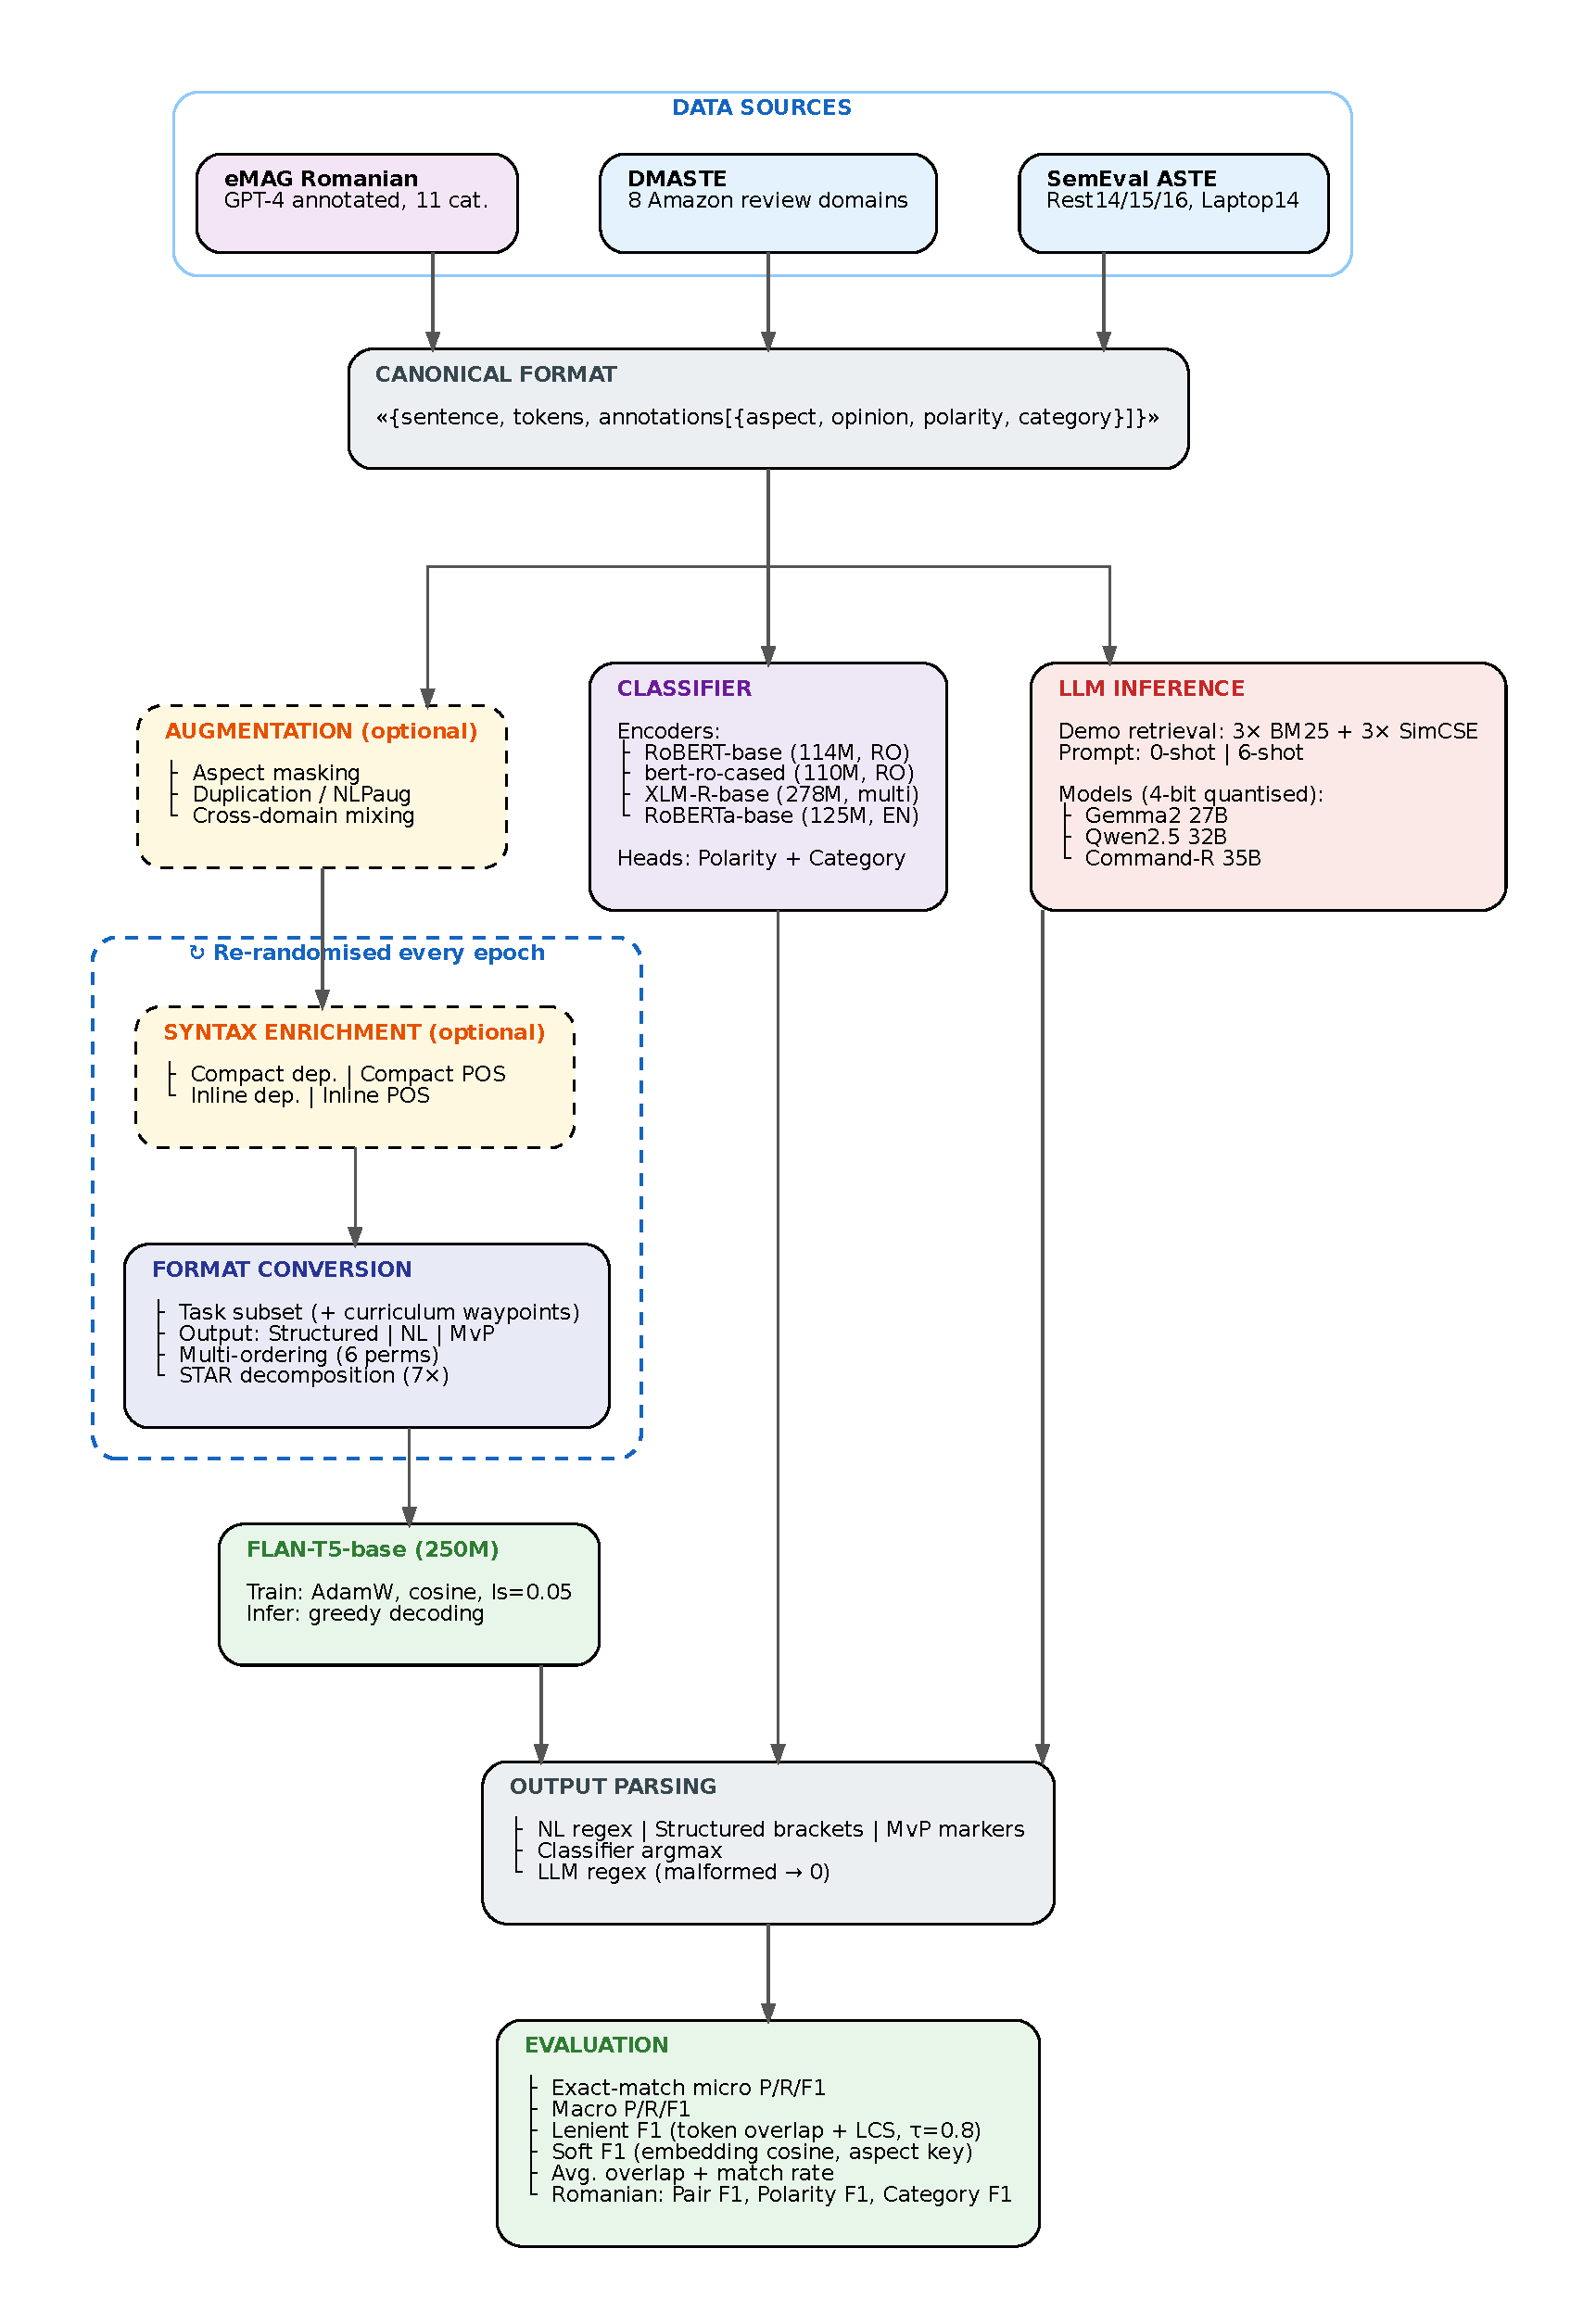
\includegraphics[width=\textwidth, height=0.88\textheight, keepaspectratio]{figures/pipeline_complete.pdf}
\caption{Training and evaluation pipeline. The dashed cluster indicates steps that are re-randomised every epoch. The three parallel evaluation paths (generative, discriminative baseline, LLM inference) are shown on the right.}
\label{fig:pipeline}
\end{figure}


\section{Datasets}

\subsection{SemEval ASTE}

The primary benchmark uses datasets from the SemEval shared tasks~\cite{pontiki2014semeval, pontiki2015semeval, pontiki2016semeval}, processed into ASTE format by Xu et al.~\cite{xu2020position}:

\begin{table}[htbp]
\centering
\caption{SemEval ASTE dataset statistics.}
\small
\begin{tabular}{@{}lrrrr@{}}
\toprule
\textbf{Dataset} & \textbf{Sentences} & \textbf{Triplets} & \textbf{Avg/sent} & \textbf{Role} \\
\midrule
Restaurant14 (train) & 1266 & 2338 & 1.85 & Train \\
Restaurant14 (test) & 492 & 994 & 2.02 & ID test \\
Restaurant15 (test) & 322 & 485 & 1.51 & Near-OOD test \\
Restaurant16 (test) & 326 & 514 & 1.58 & Near-OOD test \\
Laptop14 (test) & 328 & 543 & 1.66 & OOD test \\
\bottomrule
\end{tabular}
\end{table}

We train exclusively on Restaurant14 and test on all four. A methodological note: we discovered that 80\% of Rest15 test sentences overlap with the combined Rest14+15+16 training set (they share source Yelp reviews across SemEval years). This is why we use Rest14-only training rather than pooling all restaurant data.

\subsection{DMASTE}

The DMASTE benchmark~\cite{xu2023dmaste} provides a more rigorous cross-domain evaluation with 8 Amazon review domains:

\begin{table}[htbp]
\centering
\caption{DMASTE dataset statistics.}
\small
\begin{tabular}{@{}llrrrr@{}}
\toprule
\textbf{Role} & \textbf{Domain} & \textbf{Sentences} & \textbf{Triplets} & \textbf{Avg/sent} & \textbf{Implicit \%} \\
\midrule
Source & Electronics & 1395 & 5292 & 3.79 & 40.5\% \\
Source & Beauty & 535 & 2221 & 4.15 & 43.6\% \\
Source & Fashion & 851 & 3241 & 3.81 & 43.9\% \\
Source & Home & 1050 & 3852 & 3.67 & 42.8\% \\
\midrule
Target & Book & 325 & 1068 & 3.29 & 37.8\% \\
Target & Grocery & 353 & 1281 & 3.63 & 40.1\% \\
Target & Pet & 340 & 1104 & 3.25 & 47.4\% \\
Target & Toy & 354 & 1431 & 4.04 & 42.7\% \\
\bottomrule
\end{tabular}
\end{table}

DMASTE differs from SemEval in several ways: sentences are much longer (55--64 tokens vs 15--17), more triplets per sentence (3--4 vs 1.5--2), and 40--47\% of aspects are implicit.

\subsection{Romanian ABSA (eMAG)}

For multilingual evaluation, we use a dataset of Romanian phone reviews from eMAG (a Romanian e-commerce platform). The task is polarity and category prediction across 11 predefined categories (experience, durability, performance, battery, price\_quality, design, camera, audio, software, brand, service). The training set contains 27,630 sentences (90,778 annotations, 3.29 avg per sentence) and the test set contains 3,093 sentences (9,478 annotations). The polarity distribution is heavily skewed toward positive (72.4\%), with negative at 22.6\% and neutral at 5.0\%.

The training data was annotated with GPT-4 assistance: reviews were processed by GPT-4 to identify aspects and assign polarity/category labels from the predefined taxonomy, followed by human review. The test set was annotated independently.



\chapter{Experimental Results}\label{ch:results}

This chapter presents the experimental results across the three benchmarks. We begin with a data analysis that characterises the datasets and explains the sources of cross-domain difficulty. We then present the main finding (output format impact), followed by syntax enrichment results, the series of training strategies that did not help, the DMASTE cross-domain benchmark, LLM comparisons on English and Romanian, in-domain benchmark context, and a detailed error analysis. The chapter concludes with a discussion of the mechanisms behind our findings.

\section{Data Analysis}\label{sec:data-analysis}

Before presenting experimental results, we analyse the characteristics of the datasets to understand what makes cross-domain transfer difficult. Figure~\ref{fig:r3-polarity} shows the polarity distribution across datasets, and Figure~\ref{fig:r3-sentlen} compares sentence length distributions between the training domain (Rest14) and the OOD target (Laptop14).

The Rest14 training set contains 1266 sentences with 2338 annotations (1.85 annotations per sentence on average). Sentences are relatively short: mean 17.3 words, median 16, with 95\% of sentences under 34 words. The vocabulary is small (2916 unique words). Aspect spans are overwhelmingly single-word (mean 1.38 words) and opinion spans even shorter (mean 1.17 words). The polarity distribution is skewed toward positive (72.4\%), with negative at 20.5\% and neutral at 7.1\%.

\begin{figure}[H]
\centering
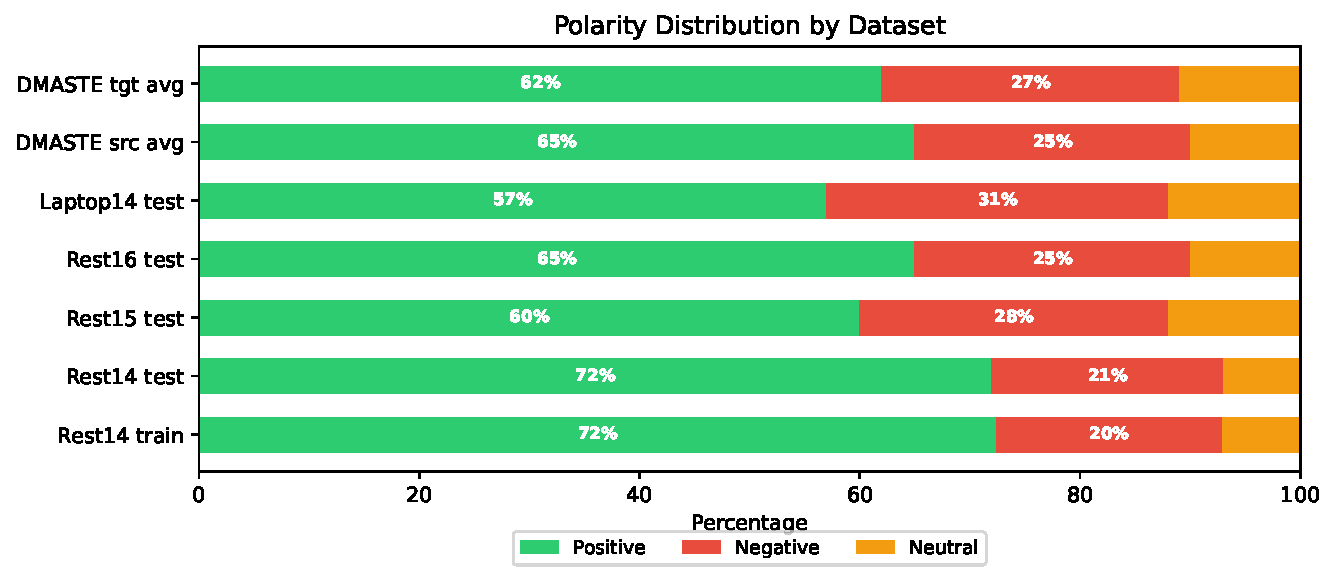
\includegraphics[width=0.95\textwidth]{figures/r3_polarity_distribution.pdf}
\caption{Polarity distribution across all datasets used in this thesis.}
\label{fig:r3-polarity}
\end{figure}

\begin{figure}[H]
\centering
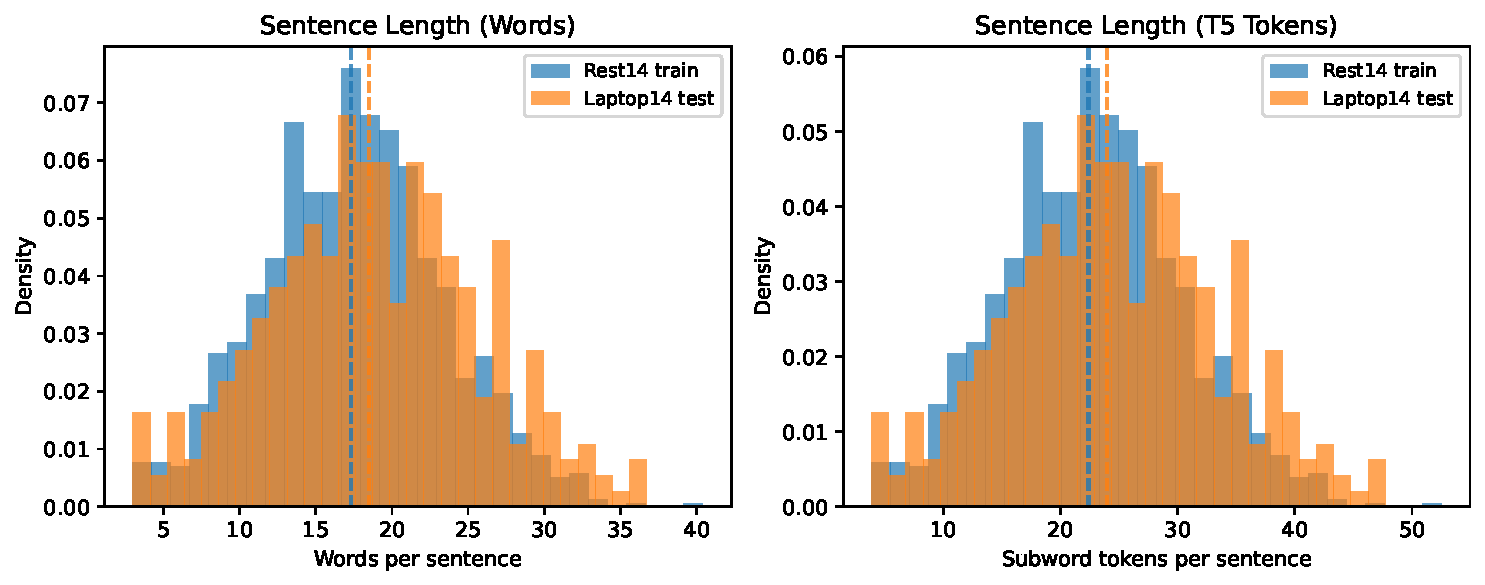
\includegraphics[width=0.95\textwidth]{figures/r3_sentence_length_histogram.pdf}
\caption{Sentence length distributions for Rest14 (training) and Laptop14 (OOD test) at word and subword token level.}
\label{fig:r3-sentlen}
\end{figure}

\subsection{Vocabulary Overlap}

Table~\ref{tab:vocab-overlap} shows token-level vocabulary overlap between training and test domains. For SemEval, only 3.7\% of Laptop14 aspect tokens appear in the Rest14 training vocabulary, while the Rest14 test set shares 31\%. Opinion overlap is higher across the board (19.7\% for Laptop14), because words like ``good'', ``terrible'', ``excellent'' appear across domains while ``pizza'' and ``keyboard'' do not.

DMASTE target domains show higher overlap overall (24--55\% aspect, 60--76\% opinion) since they share the Amazon review style with the source domains.

\begin{table}[H]
\centering
\caption{Token-level vocabulary overlap (\%) between training and test domains.}
\label{tab:vocab-overlap}
\small
\begin{tabular}{@{}llcc@{}}
\toprule
\textbf{Train} & \textbf{Test} & \textbf{Aspect overlap} & \textbf{Opinion overlap} \\
\midrule
\multicolumn{4}{l}{\textit{SemEval (Rest14 train $\rightarrow$ test sets)}} \\
\midrule
Rest14 & Rest14 (ID) & 31.0 & 33.1 \\
Rest14 & Rest15 & 20.3 & 21.7 \\
Rest14 & Rest16 & 19.6 & 24.1 \\
Rest14 & Laptop14 (OOD) & 3.7 & 19.7 \\
\midrule
\multicolumn{4}{l}{\textit{DMASTE (source domains $\rightarrow$ target domains)}} \\
\midrule
Sources & Book & 24.4 & 60.2 \\
Sources & Grocery & 38.4 & 65.3 \\
Sources & Pet & 54.5 & 75.5 \\
Sources & Toy & 41.2 & 66.8 \\
\bottomrule
\end{tabular}
\end{table}

\subsection{Linguistic Differences}

The datasets differ in their annotation styles in ways that go beyond vocabulary. Figure~\ref{fig:pos} compares the POS tag distribution for opinion spans across all datasets. The most striking difference is in opinion annotations: SemEval opinions are adjective-dominant (37--46\% of opinion head POS tags are adjectives: ``delicious'', ``horrible''), while DMASTE opinions are verb-dominant (21--24\% verbs: ``works'', ``love'', ``recommend''). This reflects different annotation conventions rather than just different vocabulary. A model trained on adjective-heavy SemEval opinions may underperform on verb-heavy DMASTE opinions regardless of vocabulary overlap.

\begin{figure}[H]
\centering
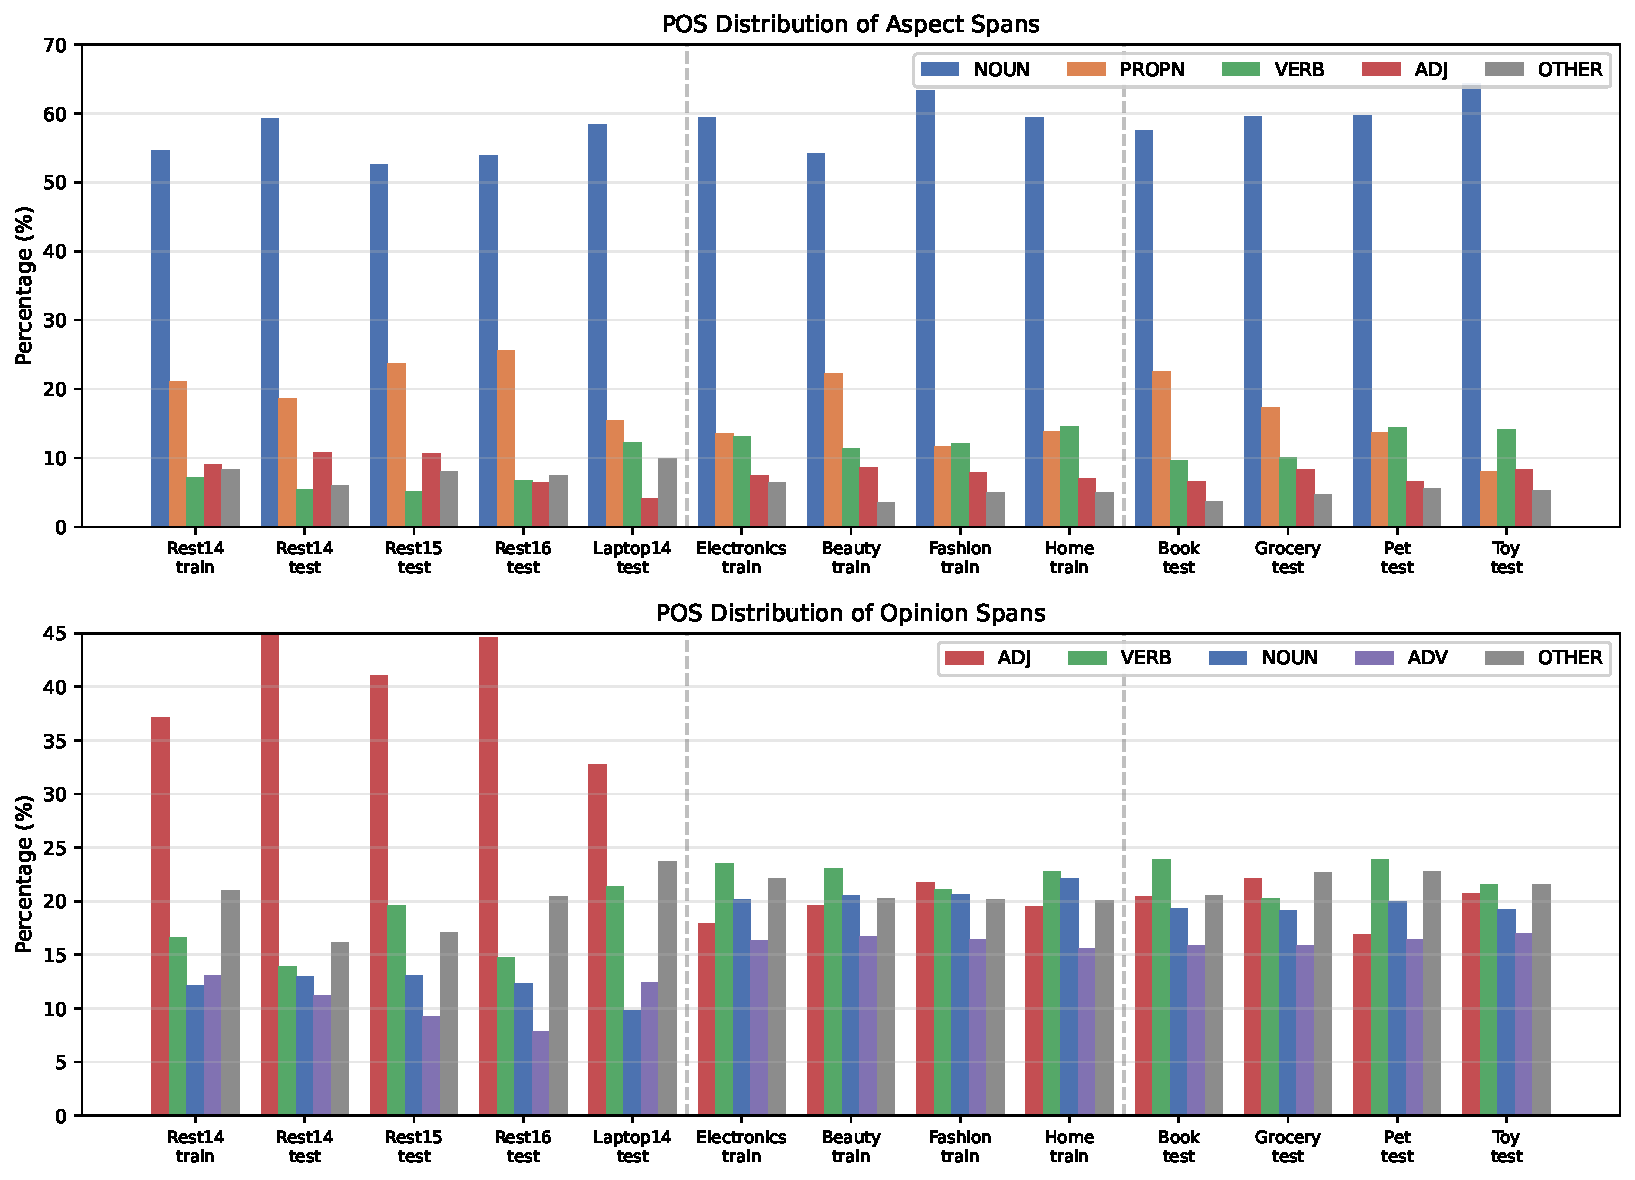
\includegraphics[width=0.95\textwidth]{figures/pos_comparison.pdf}
\caption{POS tag distribution for aspect terms (top) and opinion terms (bottom) across SemEval and DMASTE datasets.}
\label{fig:pos}
\end{figure}

\subsection{Structural Characteristics}

DMASTE sentences are 3--4$\times$ longer than SemEval (55--64 tokens vs 15--17), contain 2$\times$ more triplets per sentence (3.3--4.0 vs 1.5--2.0), and have much higher implicit aspect rates (38--47\% vs 0\% in SemEval). These compounding differences make DMASTE a substantially harder cross-domain target than the near-OOD SemEval restaurant variants.

The relationship between vocabulary overlap and performance is not straightforward. The Pet domain has the highest aspect overlap with training sources (54.5\%) but second-worst F1, explained by its 47.4\% implicit aspect rate. Vocabulary overlap is necessary but not sufficient; implicit aspects, sentence length, and annotation density all modulate the relationship.

\begin{figure}[H]
\centering
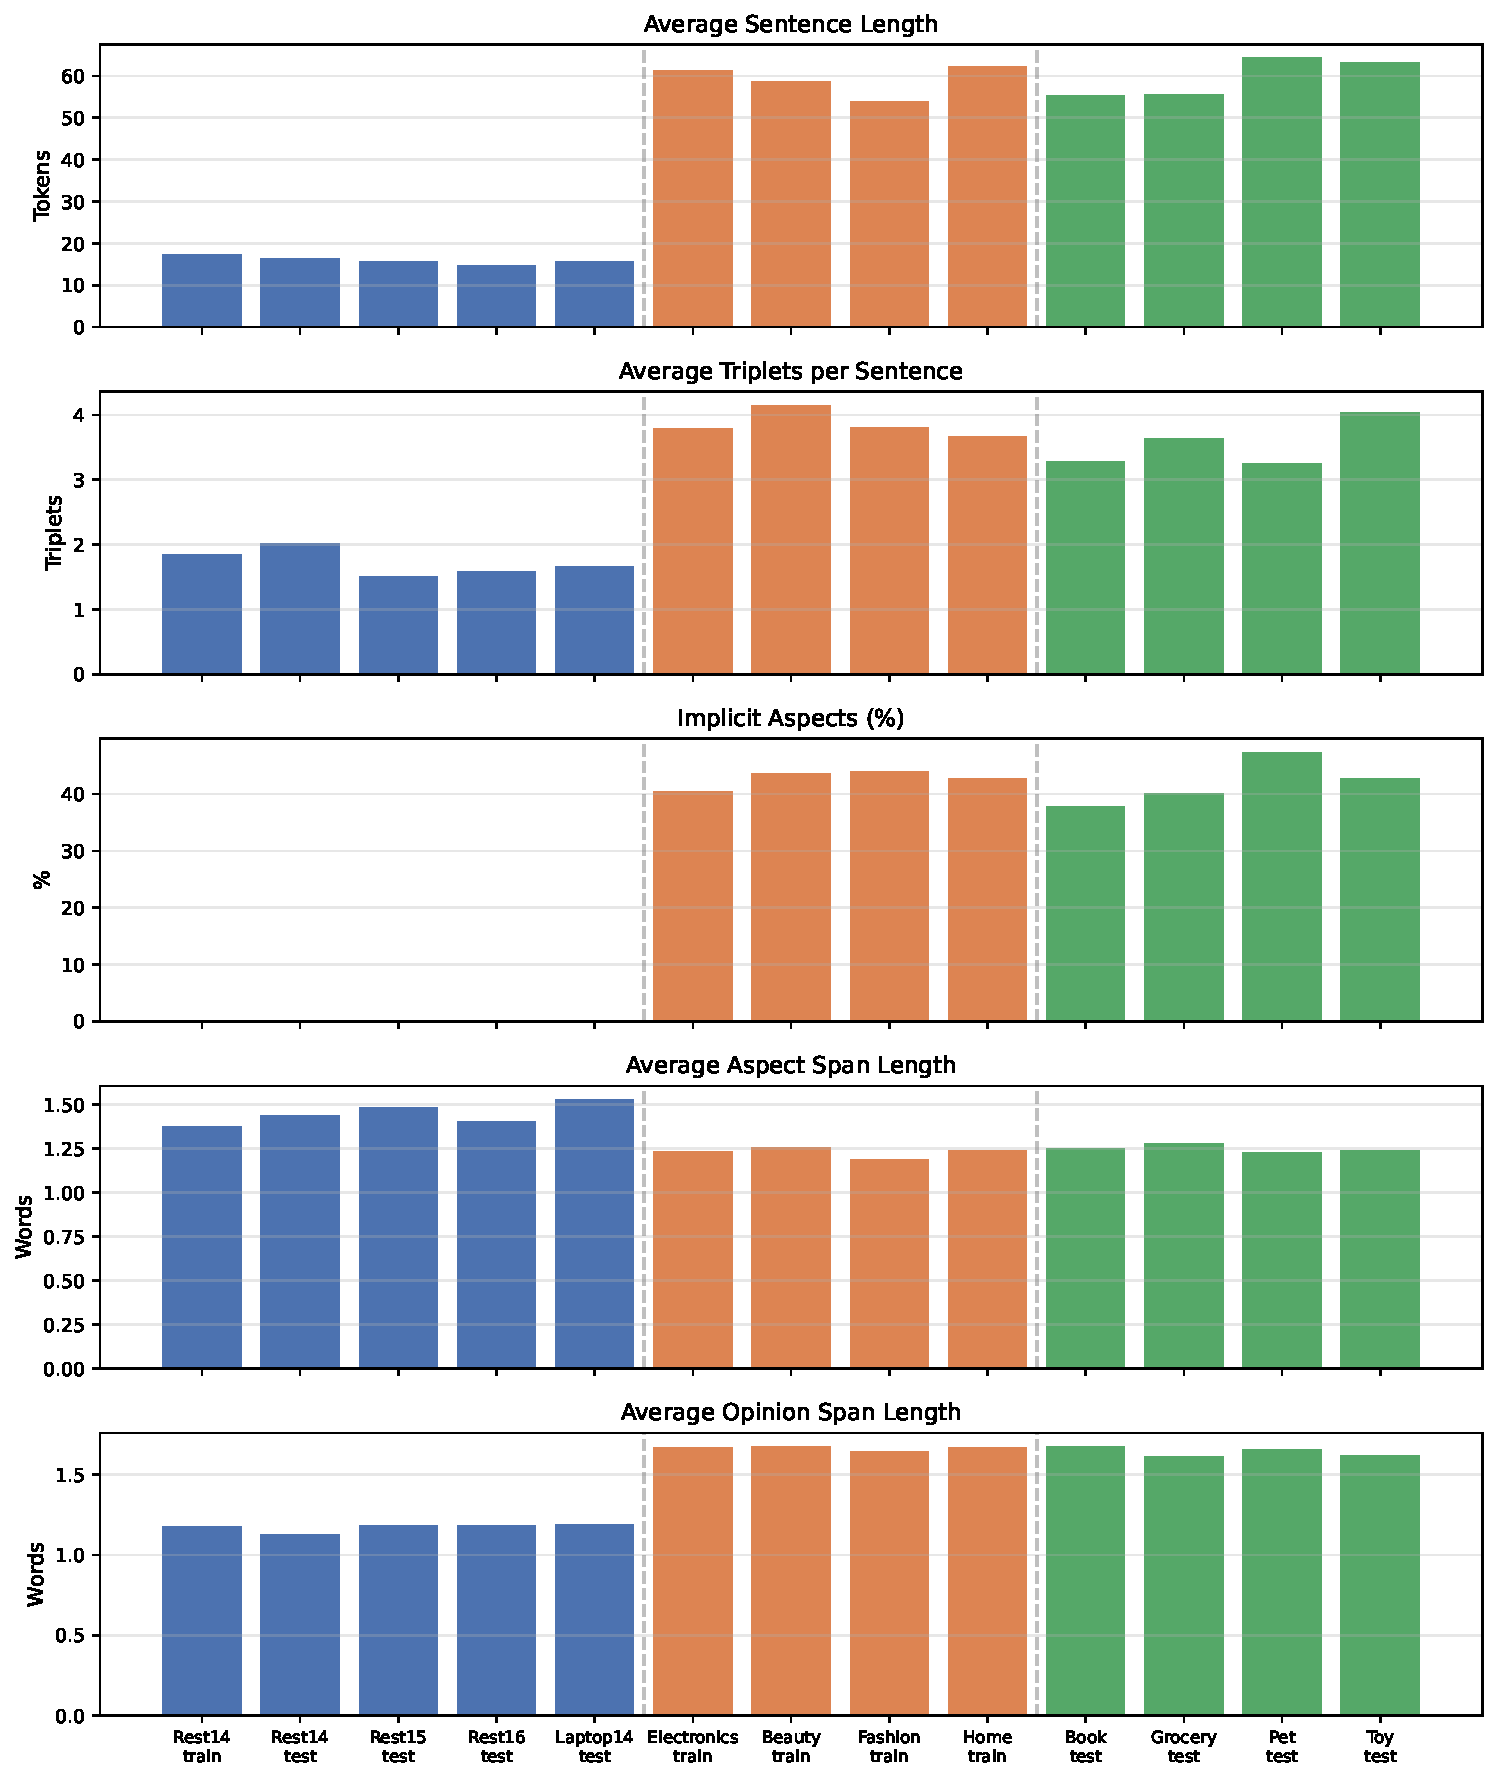
\includegraphics[width=0.95\textwidth]{figures/dataset_characteristics.pdf}
\caption{Dataset characteristics comparison: sentence length, triplets per sentence, implicit aspect rate, aspect span length, and opinion span length across all datasets.}
\label{fig:characteristics}
\end{figure}


\section{Output Format: The Main Finding}\label{sec:format-results}

Table~\ref{tab:multiseed} presents the multi-seed results (5 seeds) for the primary SemEval setup, training on Restaurant14 only.

\begin{table}[H]
\centering
\caption{Multi-seed results on SemEval ASTE (triplet micro-F1, mean$\pm$std across 5 seeds). Training on Rest14 only.}
\label{tab:multiseed}
\small
\begin{tabular}{@{}lcccc@{}}
\toprule
\textbf{Configuration} & \textbf{Rest14 (ID)} & \textbf{Rest15} & \textbf{Rest16} & \textbf{Laptop14 (OOD)} \\
\midrule
Structured baseline & 0.693$\pm$0.008 & 0.575$\pm$0.009 & 0.640$\pm$0.009 & 0.439$\pm$0.012 \\
Structured + compact dep. & 0.699$\pm$0.004 & 0.578$\pm$0.012 & 0.655$\pm$0.008 & 0.447$\pm$0.012 \\
\midrule
NL baseline & \textbf{0.722$\pm$0.005} & \textbf{0.602$\pm$0.004} & 0.680$\pm$0.010 & \textbf{0.525$\pm$0.012} \\
NL + compact dep. & 0.708$\pm$0.006 & 0.596$\pm$0.006 & 0.669$\pm$0.004 & 0.509$\pm$0.005 \\
NL + compact POS & 0.699$\pm$0.003 & 0.601$\pm$0.010 & 0.672$\pm$0.007 & 0.506$\pm$0.012 \\
NL + mixed-objective & \textbf{0.730$\pm$0.005} & 0.593$\pm$0.010 & \textbf{0.686$\pm$0.009} & 0.524$\pm$0.011 \\
\bottomrule
\end{tabular}
\end{table}

The central result: switching from structured to natural-language output provides +8.6 F1 points on Laptop14 OOD (0.439$\rightarrow$0.525), with non-overlapping confidence intervals. This is a larger improvement than any other intervention we tested. The gap widens with domain distance: +2.9 on Rest14, +2.7 on Rest15, +4.0 on Rest16, +8.6 on Laptop14.

Once the model uses NL output, adding syntax enrichment or mixed-objective training on top does not produce further gains: all NL variants land between 0.506 and 0.525 on Laptop14, within overlapping confidence intervals. We believe the format advantage comes from alignment with FLAN-T5's pre-training distribution: on OOD data where the model has less task-specific confidence, generating fluent template sentences is something it can still fall back on.

\begin{figure}[H]
\centering
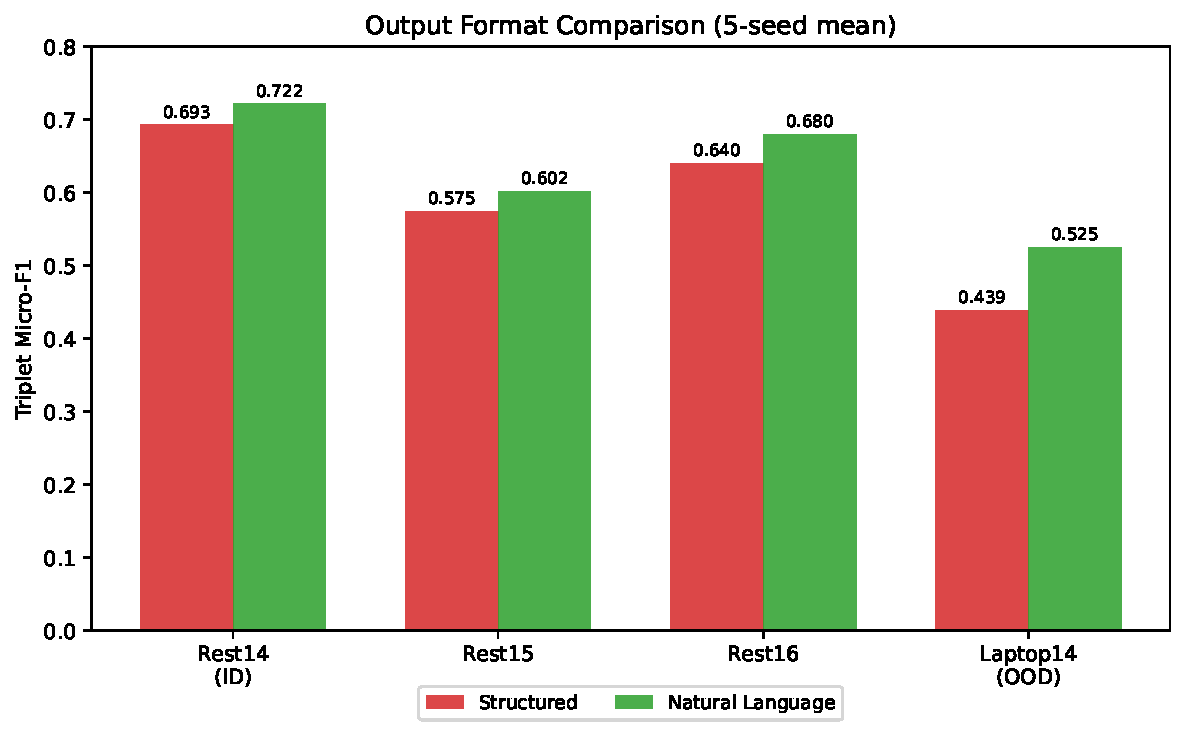
\includegraphics[width=0.85\textwidth]{figures/r3_output_format_comparison.pdf}
\caption{Output format comparison: structured vs natural-language F1 across all test sets (5-seed mean).}
\label{fig:r3-format}
\end{figure}


\section{Syntactic Enrichment}\label{sec:syntax-results}

We tested four syntax annotation modes. Only the compact dependency and compact POS modes (which add a separate Syntax line) were viable. The inline modes (which replace input tokens) consistently hurt both ID and OOD performance, likely because they corrupt the surface form the model uses for span copying.

\begin{table}[H]
\centering
\caption{Syntax modes comparison (triplet micro-F1, 20 epochs, structured format, Rest14-only training, seed 42).}
\label{tab:syntax-inline}
\small
\begin{tabular}{@{}lcc@{}}
\toprule
\textbf{Configuration} & \textbf{Rest14 (ID)} & \textbf{Laptop14 (OOD)} \\
\midrule
Baseline (no syntax) & 0.705 & 0.424 \\
+ inline dep. & 0.656 & 0.412 \\
+ inline POS & 0.660 & 0.382 \\
+ compact dep. & 0.708 & 0.481 \\
+ compact POS & 0.713 & 0.494 \\
\bottomrule
\end{tabular}
\end{table}

The multi-seed results (Table~\ref{tab:multiseed}) confirm that syntax enrichment does not significantly help OOD generalisation once the NL format is applied. The confidence intervals overlap with the NL baseline on Laptop14. We hypothesise this is data-size dependent: with Rest14-only training (1266 sentences), the additional input length from syntax annotations may dilute the signal without providing enough generalisation benefit to compensate.


\section{Training Strategies: Negative Results}\label{sec:negative}

This section documents strategies that did not reliably improve OOD performance. The ablation studies use a single random seed (42) to reduce computational cost. Single-seed results are interpreted relative to the 5-seed baseline's confidence interval (0.525$\pm$0.012 on Laptop14).

\subsection{Multi-Ordering Training and MvP/STAR Replications}\label{sec:mvp-star}

\begin{table}[H]
\centering
\caption{MvP and STAR replication results (triplet micro-F1, seed 42, Rest14-only training).}
\label{tab:mvp-star}
\small
\begin{tabular}{@{}lcccc@{}}
\toprule
\textbf{Configuration} & \textbf{Rest14} & \textbf{Rest15} & \textbf{Rest16} & \textbf{Laptop14} \\
\midrule
NL baseline (5-seed avg) & 0.722 & 0.602 & 0.680 & 0.525 \\
\midrule
MvP proper (greedy) & 0.728 & 0.605 & 0.688 & 0.528 \\
MvP proper + voting (k=3) & 0.735 & 0.604 & 0.693 & 0.530 \\
STAR proper (greedy) & 0.718 & 0.592 & 0.692 & 0.487 \\
STAR proper + voting (k=3) & 0.723 & 0.598 & 0.714 & 0.500 \\
\midrule
NL + multi-ordering (5-seed) & 0.730 & 0.593 & 0.686 & 0.524 \\
\bottomrule
\end{tabular}
\end{table}

MvP with voting achieves 0.530 on Laptop14, within the NL baseline's confidence interval. The voting mechanism helps ID compositional accuracy but does not address vocabulary or domain shift. STAR hurts OOD significantly ($-$3.8 points for greedy, $-$2.5 with voting). The pairwise sub-task decomposition multiplies training instances from the same domain without introducing any domain-relevant variation.

\subsection{Curriculum Learning}\label{sec:curriculum}

\begin{table}[H]
\centering
\caption{Curriculum learning results (triplet micro-F1, 28 epochs, NL format, Rest14 training, seed 42).}
\label{tab:curriculum}
\small
\begin{tabular}{@{}lcccc@{}}
\toprule
\textbf{Schedule} & \textbf{Rest14 (ID)} & \textbf{Rest15} & \textbf{Rest16} & \textbf{Laptop14 (OOD)} \\
\midrule
NL baseline (5-seed avg) & 0.722 & 0.602 & 0.680 & 0.525 \\
\midrule
Overlap-first & 0.716 & 0.577 & 0.670 & 0.502 \\
Fast ramp & 0.722 & 0.593 & 0.673 & 0.509 \\
Sandwich & 0.713 & 0.612 & 0.680 & 0.507 \\
\bottomrule
\end{tabular}
\end{table}

All three schedules drop Laptop14 performance by 1.6--2.3 points relative to the baseline. Curriculum schedules control the training trajectory but all data still comes from the restaurant domain. They affect how quickly the model converges on in-domain patterns, not what features it learns.

\subsection{Aspect Masking}\label{sec:masking}

\begin{table}[H]
\centering
\caption{Aspect masking results (triplet micro-F1, NL format, 28 epochs, Rest14 training, seed 42). Mask fraction = 20\%.}
\label{tab:masking}
\small
\begin{tabular}{@{}lcccc@{}}
\toprule
\textbf{Configuration} & \textbf{Rest14 (ID)} & \textbf{Rest15} & \textbf{Rest16} & \textbf{Laptop14 (OOD)} \\
\midrule
NL baseline (5-seed avg) & 0.722 & 0.602 & 0.680 & 0.525 \\
\midrule
Mask 20\% & 0.710 & 0.598 & 0.671 & 0.518 \\
Mask 20\% + dep. & 0.705 & 0.598 & 0.675 & 0.511 \\
\bottomrule
\end{tabular}
\end{table}

Masking consistently hurts. The premise was that forcing the model to predict aspects from context would improve generalisation to novel aspects. In practice, removing real aspect context removes the very signal the model needs. During training on restaurant data, the model learns to infer masked aspects from surrounding restaurant vocabulary, reinforcing domain-specific priors rather than building domain-general representations.

\subsection{Cross-Domain Data Mixing}\label{sec:domainmix}

\begin{table}[H]
\centering
\caption{Domain mixing results (triplet micro-F1, Rest14 + DMASTE domain fraction, seed 42).}
\label{tab:domainmix}
\small
\begin{tabular}{@{}lcccc@{}}
\toprule
\textbf{Mixed domain} & \textbf{Rest14} & \textbf{Rest15} & \textbf{Rest16} & \textbf{Laptop14} \\
\midrule
None (baseline) & 0.727 & 0.607 & 0.672 & 0.543 \\
\midrule
+ Beauty & 0.707 & 0.610 & 0.699 & 0.523 \\
+ Electronics & 0.720 & 0.605 & 0.685 & 0.526 \\
+ Fashion & 0.709 & 0.589 & 0.689 & 0.502 \\
+ Home & 0.736 & 0.596 & 0.689 & 0.525 \\
+ All four & 0.719 & 0.615 & 0.668 & 0.522 \\
\bottomrule
\end{tabular}
\end{table}

No domain mix improves Laptop14 OOD: all fall within the baseline confidence interval. Adding all four DMASTE domains helps near-OOD (Rest15: 0.615) but not far-OOD. The DMASTE domains share annotation conventions and sentence structure with each other but differ substantially from SemEval. Adding more Amazon-style data diversifies product vocabulary but does not bridge the structural gap to SemEval laptop reviews.

\subsection{Opinion Synonym Augmentation}

\begin{table}[H]
\centering
\caption{LLM-generated opinion synonym augmentation (Gemma2:27b).}
\label{tab:opinion-aug}
\small
\begin{tabular}{@{}lcccc@{}}
\toprule
\textbf{Fraction} & \textbf{Rest14} & \textbf{Rest15} & \textbf{Rest16} & \textbf{Laptop14} \\
\midrule
0 (NL baseline, 5-seed) & 0.722 & 0.602 & 0.680 & 0.525 \\
0.2 & 0.707 & 0.575 & 0.672 & 0.486 \\
1.0 & 0.703 & 0.571 & 0.660 & 0.472 \\
\bottomrule
\end{tabular}
\end{table}

Both augmentation fractions hurt performance across the board. Even 20\% synthetic data degrades OOD from 0.525 to 0.486. The LLM-generated sentences introduce distributional mismatch (different sentence structures, tokenisation patterns) that the model learns as noise.

\subsection{Decoding Strategies}\label{sec:decoding}

\begin{table}[H]
\centering
\caption{Decoding strategies evaluated on the NL + compact dep.\ checkpoint (seed 42).}
\label{tab:decoding}
\small
\begin{tabular}{@{}lcc@{}}
\toprule
\textbf{Strategy} & \textbf{Rest14 (ID)} & \textbf{Laptop14 (OOD)} \\
\midrule
Greedy (default) & 0.708 & 0.541 \\
Beam search (k=4) & 0.713 & 0.530 \\
Sampling (t=0.7) & 0.699 & 0.477 \\
Sampling (t=0.9) & 0.672 & 0.446 \\
Voting (5$\times$, t=0.8) & 0.710 & 0.520 \\
Constrained decoding & 0.699 & 0.483 \\
\bottomrule
\end{tabular}
\end{table}

Greedy decoding is optimal for OOD. Temperature sampling introduces noise that compounds on OOD data where the model is already less certain. Constrained decoding (FSM-based template enforcement) is unnecessary since the NL format already provides strong implicit constraints during training.

\begin{figure}[H]
\centering
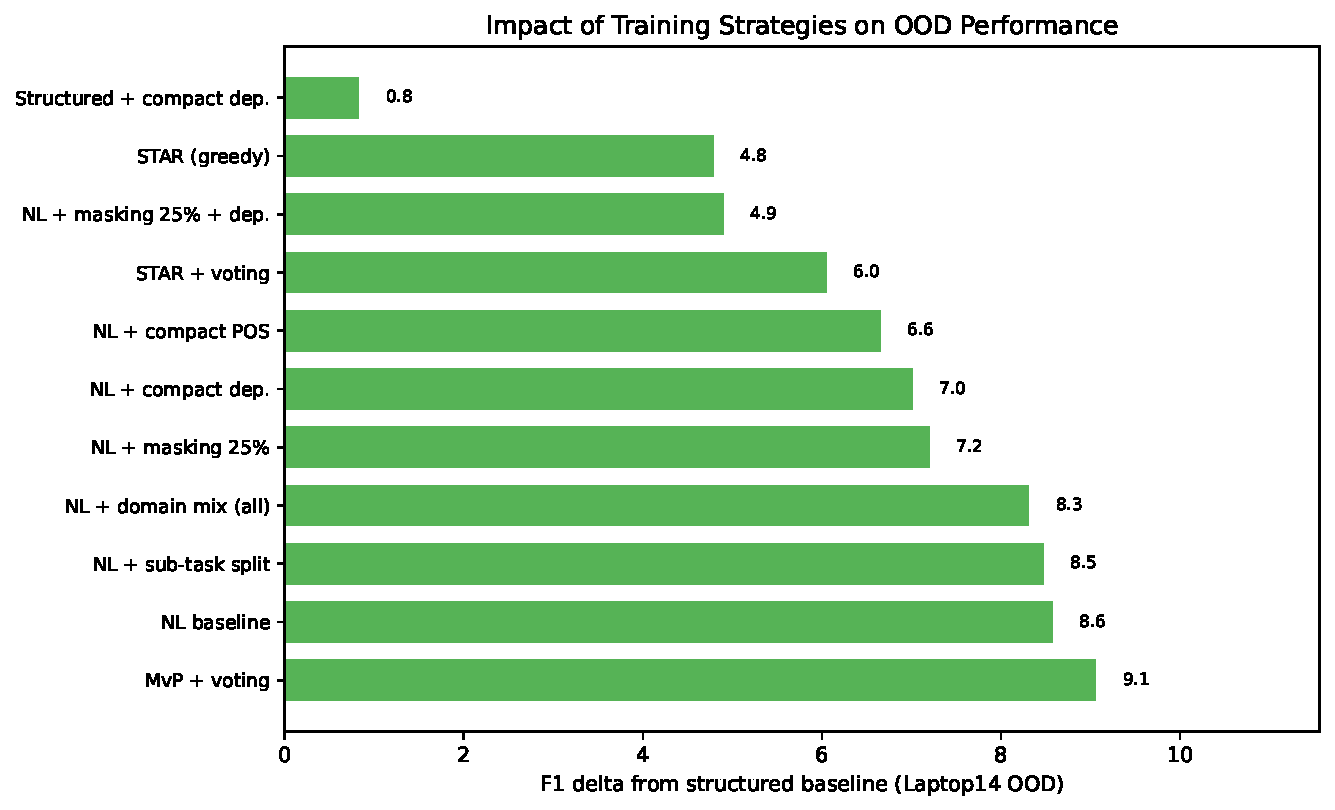
\includegraphics[width=0.95\textwidth]{figures/r3_negative_results_tornado.pdf}
\caption{F1 improvement over the structured baseline for each training strategy on Laptop14 (OOD). The NL format provides the largest gain; no further strategy adds reliably on top of it.}
\label{fig:tornado-ood}
\end{figure}

\begin{figure}[H]
\centering
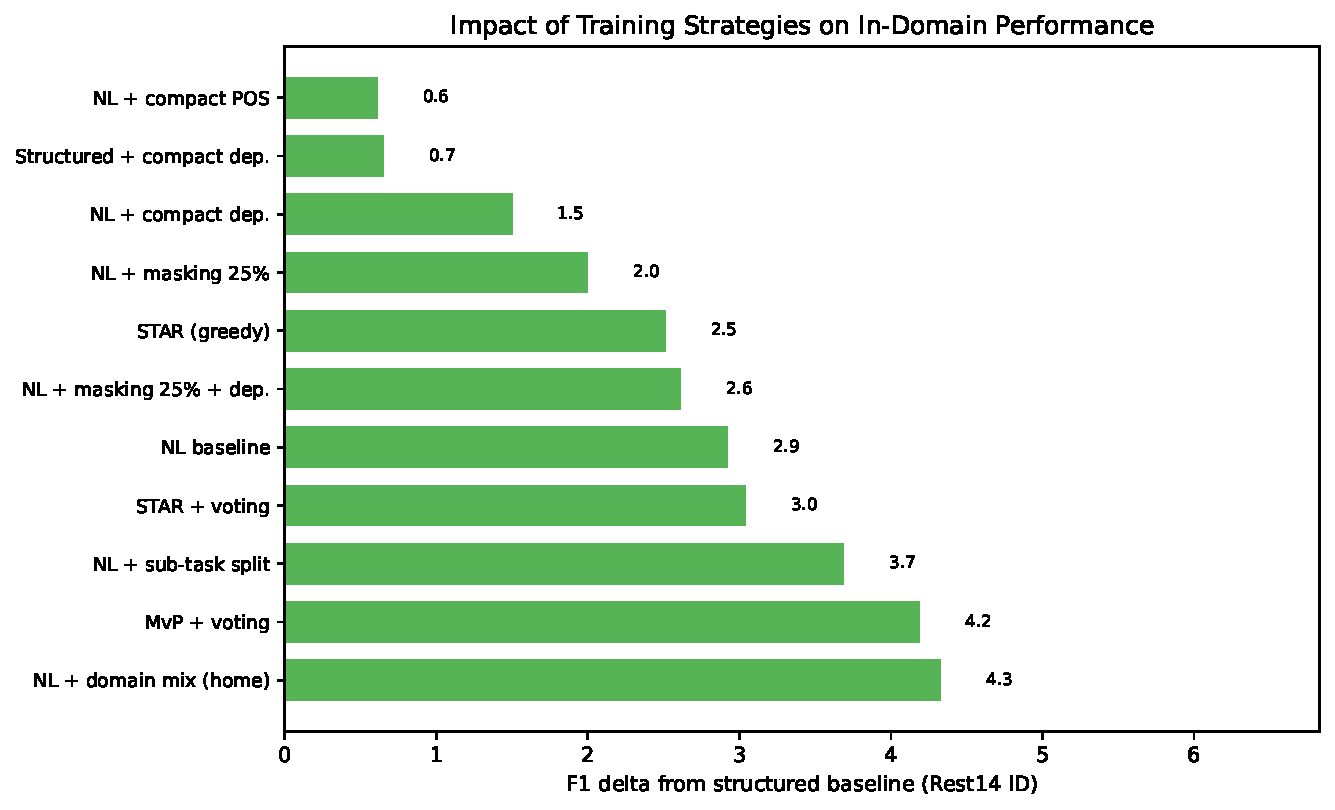
\includegraphics[width=0.95\textwidth]{figures/r3_id_results_tornado.pdf}
\caption{F1 improvement over the structured baseline for each training strategy on Rest14 (ID). Most NL-based strategies provide 2--4 F1 points of improvement.}
\label{fig:tornado-id}
\end{figure}


\section{DMASTE Cross-Domain Benchmark}\label{sec:dmaste}

Table~\ref{tab:dmaste} presents results on the DMASTE benchmark, which provides a more rigorous cross-domain evaluation with 4 target domains held out entirely from training.

\begin{table}[H]
\centering
\caption{DMASTE cross-domain results (triplet micro-F1, single seed).}
\label{tab:dmaste}
\small
\begin{tabular}{@{}lccccc@{}}
\toprule
\textbf{Method} & \textbf{Book} & \textbf{Grocery} & \textbf{Pet} & \textbf{Toy} & \textbf{Avg} \\
\midrule
\multicolumn{6}{l}{\textit{Single-source (Electronics $\rightarrow$ target)}} \\
\midrule
Structured & 34.49 & 38.88 & 37.62 & 44.67 & 38.92 \\
NL baseline & 36.05 & 43.65 & 38.93 & 46.74 & 41.34 \\
NL + multi-ordering & 37.28 & 43.78 & 40.33 & 46.72 & 42.03 \\
NL + compact dep. & 34.74 & 42.45 & 38.47 & 44.77 & 40.11 \\
RoBERTa (span) & 10.59 & 16.08 & 15.35 & 13.95 & 13.99 \\
\midrule
GAS$^\dagger$~\cite{zhang2021towards} & 35.57 & 39.16 & 38.17 & 43.55 & 39.11 \\
Span-ASTE$^\dagger$~\cite{xu2021learning} & \textbf{40.36} & \textbf{45.36} & \textbf{41.04} & \textbf{47.23} & \textbf{43.50} \\
\midrule
\multicolumn{6}{l}{\textit{Multi-source (All 4 sources $\rightarrow$ target)}} \\
\midrule
Structured & 37.50 & 44.96 & 42.47 & 47.33 & 43.07 \\
NL baseline & 41.27 & 46.62 & 43.22 & 50.16 & 45.32 \\
NL + multi-ordering & \textbf{41.83} & \textbf{46.90} & 43.06 & 50.02 & \textbf{45.45} \\
NL + compact dep. & 40.45 & 46.47 & \textbf{43.77} & 48.56 & 44.81 \\
RoBERTa (span) & 20.39 & 23.16 & 22.37 & 22.15 & 22.02 \\
\midrule
Span-ASTE$^\dagger$~\cite{xu2021learning} & \textbf{41.83} & 46.07 & 43.62 & \textbf{50.16} & 45.42 \\
\bottomrule
\multicolumn{6}{l}{\small $^\dagger$ Results as reported by Xu et al.~\cite{xu2023dmaste}.}
\end{tabular}
\end{table}

In the multi-source setting, our NL models (45.32--45.45 avg) match Span-ASTE (45.42), the best result reported in the DMASTE paper. This is achieved without any domain adaptation, using a simple FLAN-T5-base model with NL output. In single-source, we outperform GAS (+3 avg F1) and approach Span-ASTE ($-$1.5 avg).

The NL format advantage over structured output (+2.3 avg in multi-source) is smaller than on SemEval (+8.6) but consistent. The RoBERTa span baseline generalises very poorly (14--22 avg), confirming that the naive discriminative approach fundamentally lacks cross-domain transfer capability.

\begin{figure}[H]
\centering
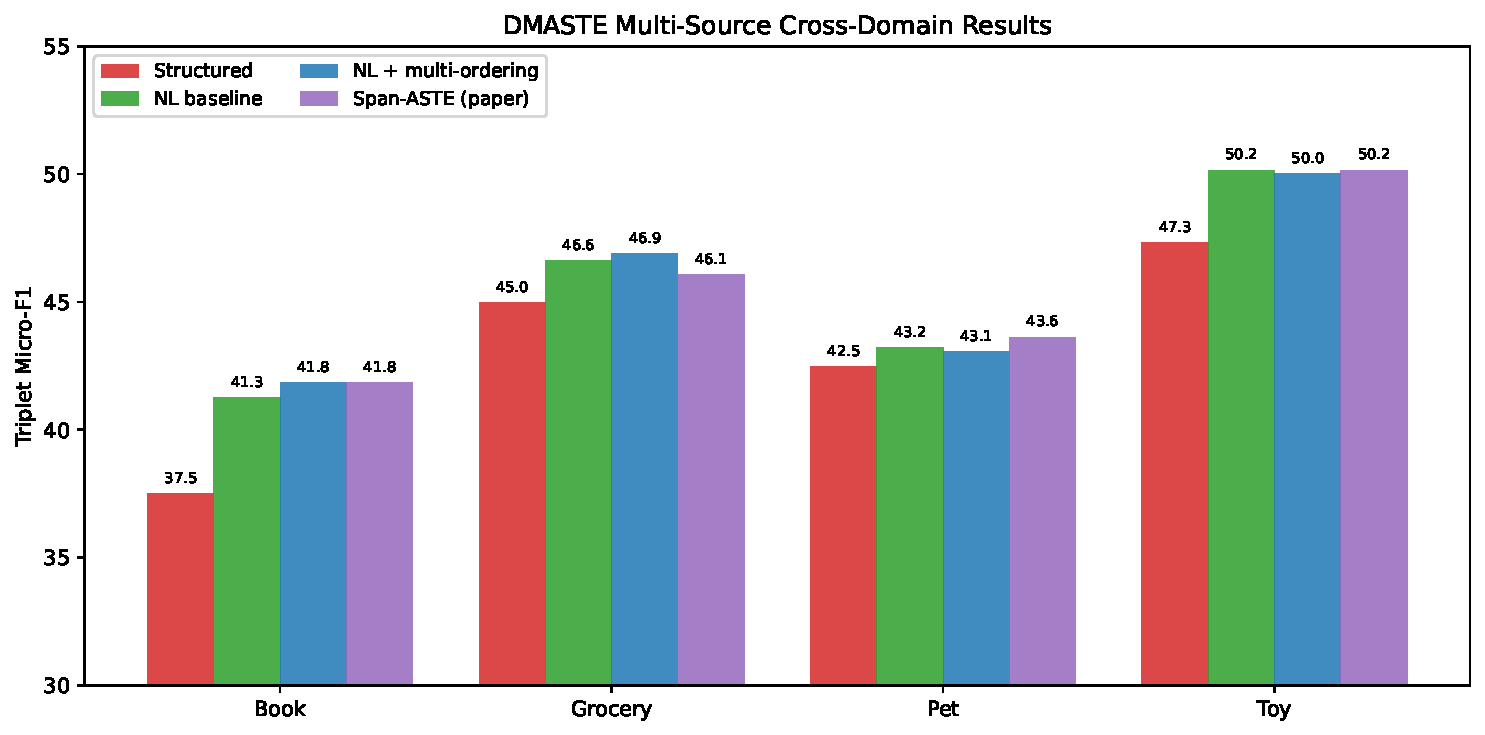
\includegraphics[width=0.95\textwidth]{figures/r3_dmaste_comparison.pdf}
\caption{DMASTE multi-source cross-domain results by method and target domain.}
\label{fig:r3-dmaste}
\end{figure}


\section{LLM Comparison on English ASTE}\label{sec:llm-english}

Table~\ref{tab:llm-semeval} presents LLM results on the SemEval ASTE benchmark alongside our fine-tuned baselines.

\begin{table}[H]
\centering
\caption{Cross-method comparison on SemEval ASTE (triplet micro-F1). LLMs use per-dataset demonstrations for 6-shot.}
\label{tab:llm-semeval}
\small
\begin{tabular}{@{}lrcccc@{}}
\toprule
\textbf{Method} & \textbf{Params} & \textbf{Rest14} & \textbf{Rest15} & \textbf{Rest16} & \textbf{Laptop14} \\
\midrule
\multicolumn{6}{l}{\textit{LLMs (few-shot, no fine-tuning)}} \\
\midrule
Gemma2 27B 0-shot & 27B & 0.441 & 0.418 & 0.455 & 0.275 \\
Gemma2 27B 6-shot & 27B & 0.646 & 0.592 & 0.637 & 0.410 \\
Qwen2.5 32B 0-shot & 32B & 0.535 & 0.451 & 0.556 & 0.363 \\
Qwen2.5 32B 6-shot & 32B & 0.603 & 0.527 & 0.614 & 0.370 \\
Command-R 0-shot & 35B & 0.318 & 0.256 & 0.309 & 0.206 \\
Command-R 6-shot & 35B & 0.576 & 0.499 & 0.568 & 0.373 \\
\midrule
\multicolumn{6}{l}{\textit{Fine-tuned models}} \\
\midrule
RoBERTa span (ours) & 125M & 0.544 & 0.461 & 0.560 & 0.379 \\
T5 structured & 250M & 0.693 & 0.575 & 0.640 & 0.439 \\
T5 NL baseline & 250M & \textbf{0.722} & \textbf{0.602} & \textbf{0.680} & \textbf{0.525} \\
\bottomrule
\end{tabular}
\end{table}

The fine-tuned T5 with NL output (250M) outperforms all LLMs on every test set, despite being 100$\times$ smaller than the largest model tested. The gap is particularly large on OOD data: 0.525 vs 0.410 for the best LLM (Gemma2 27B 6-shot) on Laptop14, a difference of 11.5 F1 points.

Among the LLMs, Gemma2 27B with 6-shot demonstrations performs best across all datasets. The advantage provided by the few-shot setting is substantial, especially for Gemma2 and Command-R, that benefit from an average increase in F1 score of 0.174 and 0.258 respectively. Interestingly, although in the Laptop14 few-shot evaluation the 6 examples presented to the models were picked from the Rest14 dataset (to simulate OOD testing), the drop in performance between few-shot and 0-shot did not increase compared to in-domain, suggesting that the LLMs were not particularly affected by the vocabulary shift in the demonstrations.

Our naive RoBERTa span baseline (125M, fine-tuned) performs comparably to the LLMs in 6-shot on Laptop14 (0.379 vs 0.370--0.410). The fine-tuned T5 structured baseline (250M) outperforms all LLMs even without the NL format advantage. This suggests that for structured extraction tasks, task-specific fine-tuning remains more effective than in-context learning at the 27--35B parameter scale.

\begin{figure}[H]
\centering
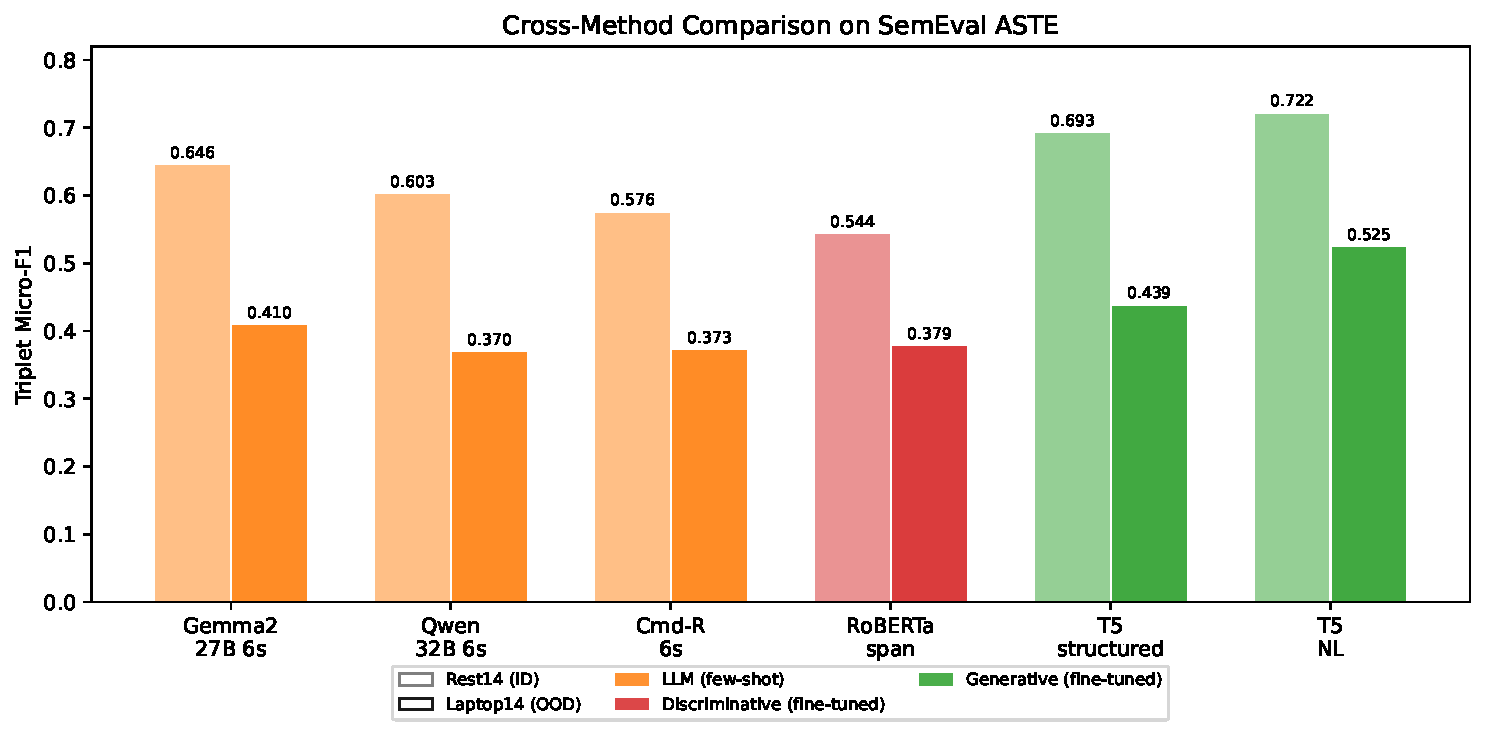
\includegraphics[width=0.95\textwidth]{figures/r4_crossmethod_english.pdf}
\caption{Cross-method comparison on SemEval ASTE: LLMs (few-shot) vs fine-tuned models, showing both in-domain (Rest14) and out-of-domain (Laptop14) performance.}
\label{fig:crossmethod}
\end{figure}


\section{Romanian ABSA}\label{sec:romanian}

Figures~\ref{fig:r4-polarity}--\ref{fig:r4-sentlen} characterise the Romanian eMAG dataset. The polarity distribution is heavily skewed toward positive (72.4\%), similar to the English SemEval data. Sentences are considerably longer than in English SemEval: mean 43.5 words (median 23), with a long tail reaching up to 309 words. At the subword token level (T5 tokenizer), the mean is 73.6 tokens (median 39, P95 = 266). The most frequent category is ``experience'' (25.7\%), followed by ``performance'' (11.5\%) and ``battery'' (10.3\%).

\begin{figure}[H]
\centering
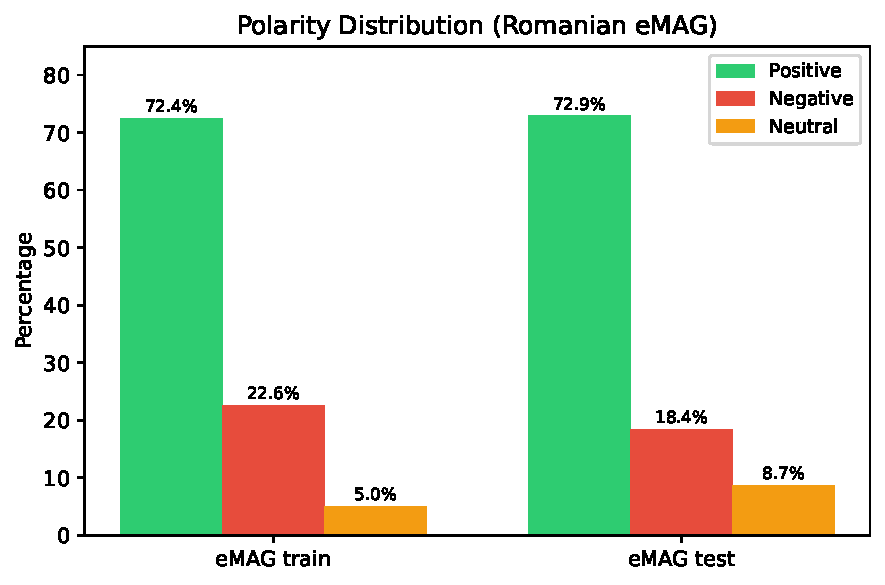
\includegraphics[width=0.7\textwidth]{figures/r4_polarity_distribution.pdf}
\caption{Polarity distribution in the Romanian eMAG training and test sets.}
\label{fig:r4-polarity}
\end{figure}

\begin{figure}[H]
\centering
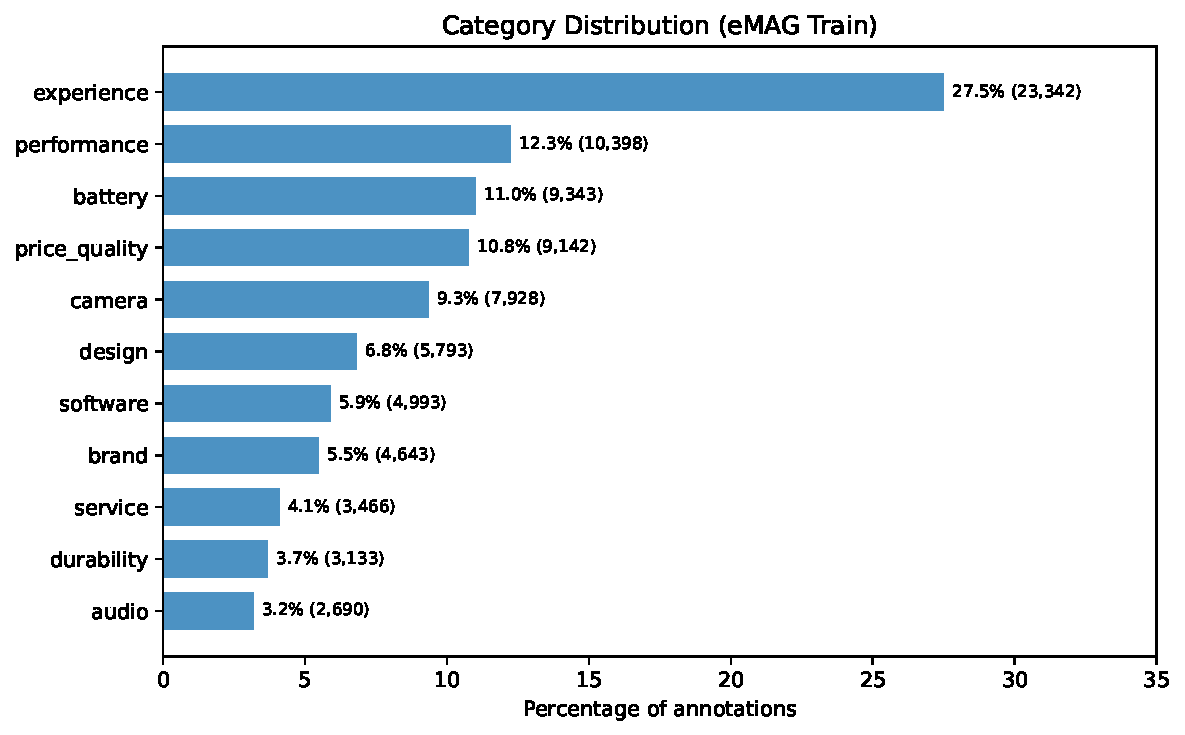
\includegraphics[width=0.85\textwidth]{figures/r4_category_distribution.pdf}
\caption{Category distribution in the Romanian eMAG training set (11 classes).}
\label{fig:r4-categories}
\end{figure}

\begin{figure}[H]
\centering
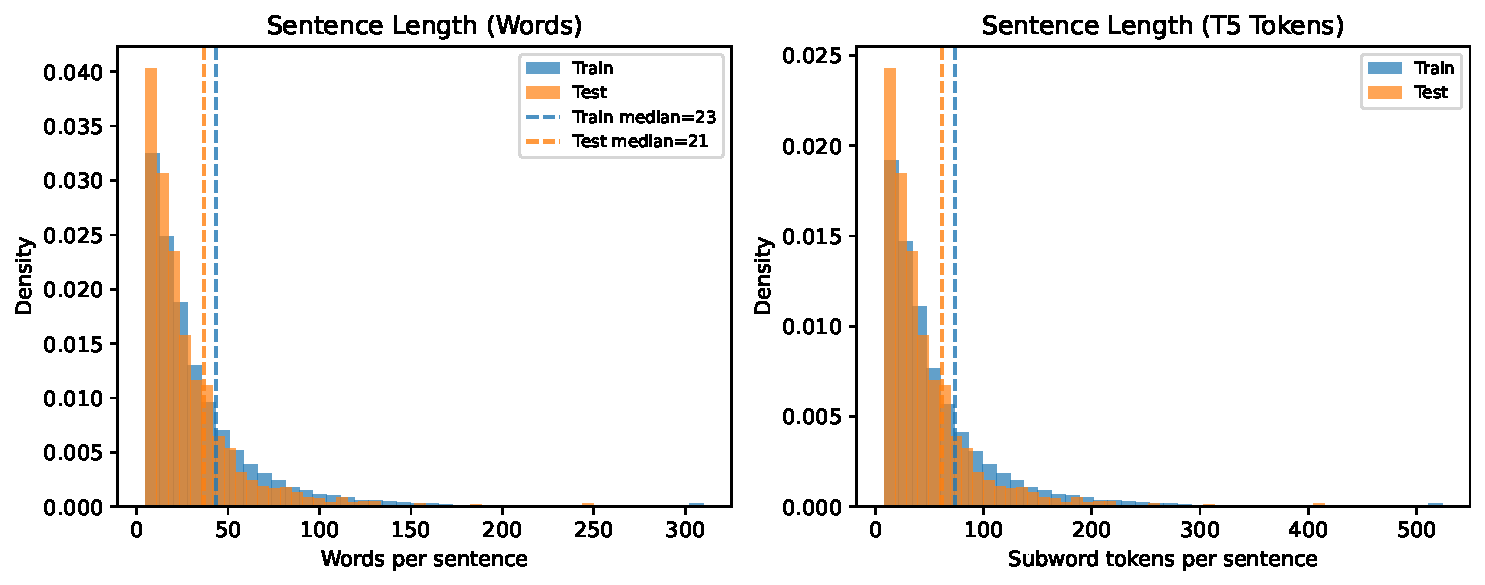
\includegraphics[width=0.95\textwidth]{figures/r4_sentence_length_histogram.pdf}
\caption{Sentence length distributions for the Romanian eMAG dataset at word and subword token level.}
\label{fig:r4-sentlen}
\end{figure}

\begin{table}[H]
\centering
\caption{Romanian ABSA results on eMAG phone reviews. Pair F1 = polarity + category must both match.}
\label{tab:romanian}
\small
\begin{tabular}{@{}lrccc@{}}
\toprule
\textbf{Method} & \textbf{Params} & \textbf{Pair F1} & \textbf{Polarity F1} & \textbf{Category F1} \\
\midrule
\multicolumn{5}{l}{\textit{LLMs (few-shot, no fine-tuning)}} \\
\midrule
Gemma2 27B 0-shot & 27B & 0.745 & \textbf{0.888} & 0.804 \\
Gemma2 27B 6-shot & 27B & 0.758 & \textbf{0.888} & 0.826 \\
Qwen2.5 32B 0-shot & 32B & 0.621 & 0.854 & 0.689 \\
Qwen2.5 32B 6-shot & 32B & 0.740 & 0.881 & 0.807 \\
Command-R 0-shot & 35B & 0.535 & 0.766 & 0.612 \\
Command-R 6-shot & 35B & 0.750 & 0.880 & 0.821 \\
\midrule
\multicolumn{5}{l}{\textit{Fine-tuned models}} \\
\midrule
RoBERT-base (RO) & 114M & 0.792 & 0.878 & \textbf{0.862} \\
bert-base-ro-cased & 110M & 0.793 & 0.877 & 0.858 \\
XLM-R-base & 278M & \textbf{0.795} & 0.881 & 0.861 \\
FLAN-T5-base (NL) & 250M & 0.764 & 0.882 & 0.853 \\
\bottomrule
\end{tabular}
\end{table}

Polarity classification is easy for all methods (0.85--0.89 F1), with only 0-shot Command-R scoring under 0.85. The bottleneck is category prediction, where LLMs score 0.61--0.83 while fine-tuned models achieve 0.85--0.86. We believe this is due to the taxonomy (11 classes) being specific to this dataset and not something LLMs would have encountered during pre-training. The 6-shot examples help LLMs learn the taxonomy, enabling a jump of roughly 0.2 in Category F1 for Command-R, but they still fall short of fine-tuned models that have seen the full training set.

XLM-R-base achieves the best pair F1 (0.795), followed closely by the monolingual Romanian models: bert-base-romanian-cased (0.793) and RoBERT-base (0.792). FLAN-T5-base trails slightly (0.764). All fine-tuned models outperform all LLMs on pair F1 by an average of roughly 0.1.

Gemma2 stands out: in 0-shot it achieves 0.745 pair F1 without any task-specific data, nearly matching the fine-tuned FLAN-T5. Interestingly, Gemma2 is by far the most English-centric of the three, its training data being primarily English~\cite{team2024gemma}. By contrast, Qwen2.5 is reported to have been trained on more than 29 languages including Romanian~\cite{hui2024qwen2}, and Command-R on 10 major languages, although Romanian was not included~\cite{cohere2024commandr}.

The monolingual Romanian models (110--114M) perform within 0.3 F1 points of XLM-R-base (278M) despite being 2.5$\times$ smaller. This is consistent with the ``curse of multilinguality''~\cite{chang2023multilinguality}: XLM-R distributes its capacity across 100 languages, while RoBERT dedicates all capacity to Romanian. Bérard et al.~\cite{berard2026capacity} confirmed this empirically, showing that multilingual language models consistently underperform monolingual counterparts due to capacity constraints. XLM-R-base (278M parameters) distributes its capacity across 100 languages, meaning Romanian gets a fraction of the total representational budget. RoBERT-base (114M parameters) dedicates all its capacity to Romanian, having been trained on 12GB of exclusively Romanian text. The result is that per-parameter efficiency for Romanian is much higher in the monolingual model.

This finding is not specific to Romanian. Velankar et al.~\cite{velankar2022mono} demonstrated the same pattern for Marathi: monolingual Marathi BERT models outperformed XLM-RoBERTa on five downstream tasks despite the multilingual model being substantially larger. Hasan et al.~\cite{tanvir2023bangla} reported consistent findings for Bangla sentiment analysis.

In our results, XLM-R does still slightly outperform the monolingual models (0.795 vs 0.792--0.793). This small advantage may come from cross-lingual transfer: XLM-R has seen sentiment-related patterns across many languages during pre-training. The difference is small enough (0.2--0.3 F1 points) that it would likely disappear with multi-seed evaluation. For practical purposes, the monolingual and multilingual models are equivalent on this task.

The practical implication is that for Romanian ABSA classification, a 110M monolingual model provides essentially the same performance as a 278M multilingual model at lower computational cost. This matters for deployment: the monolingual model is faster to fine-tune, requires less memory at inference, and achieves the same result.

FLAN-T5-base trails by 3 points despite being a 250M model. This is expected: it is an English-centric generative model being asked to perform a classification task in a language it was not primarily trained on. That it still achieves 0.764, outperforming all LLMs, demonstrates that even modest fine-tuning on target-language data is effective. But for this particular task (classification with a fixed taxonomy), the encoder-based classifiers with language-appropriate pre-training have a natural architectural advantage.

Interestingly, among the LLMs, the relationship between language coverage and performance appears to reverse. Gemma2, the most English-centric of the three (trained on 13 trillion tokens of primarily English web data~\cite{team2024gemma}), outperforms both Qwen2.5 (29+ languages including Romanian~\cite{hui2024qwen2}) and Command-R (10 languages~\cite{cohere2024commandr}) on Romanian text. Kapo\v{c}i\={u}t\.{e}-Dzikien\.{e} et al.~\cite{kapociute2025baltic} observed a similar pattern when evaluating open-weight LLMs on Baltic languages, where Gemma~2 performed close to top commercial models while explicitly multilingual LLMs struggled. The explanation likely lies in the task structure: the system prompt, category labels, and polarity names are all in English; only the review text is in Romanian. Recent work has shown that English-dominant LLMs convert non-English input into English-like internal representations in their early layers and perform reasoning in an English-aligned concept space before routing back to the target language~\cite{wendler2024llamas, zhao2024multilingualism, schut2025multilingual}. Since our task requires no non-English output, a model that concentrates all its capacity on English might have stronger representations precisely where the task demands them.

\begin{figure}[H]
\centering
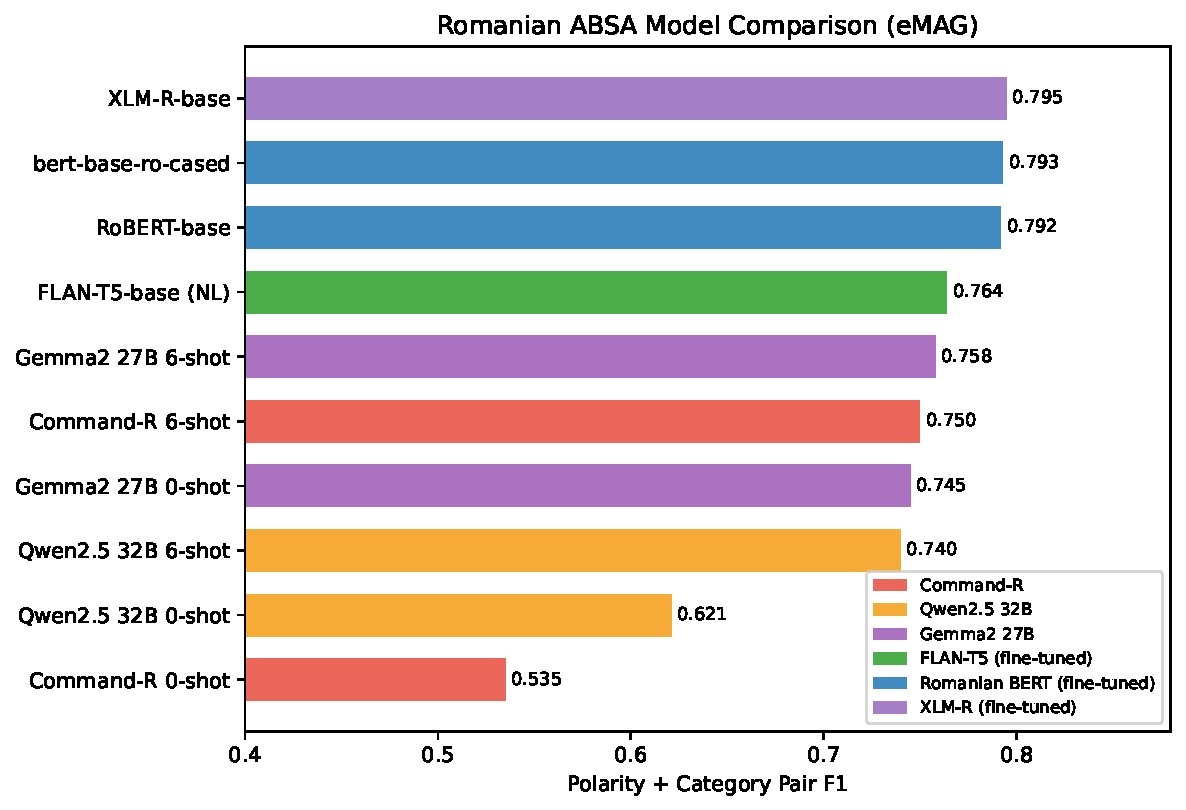
\includegraphics[width=0.85\textwidth]{figures/r4_romanian_comparison.pdf}
\caption{Romanian ABSA model comparison: all models ranked by polarity + category pair F1.}
\label{fig:romanian}
\end{figure}

\begin{figure}[H]
\centering
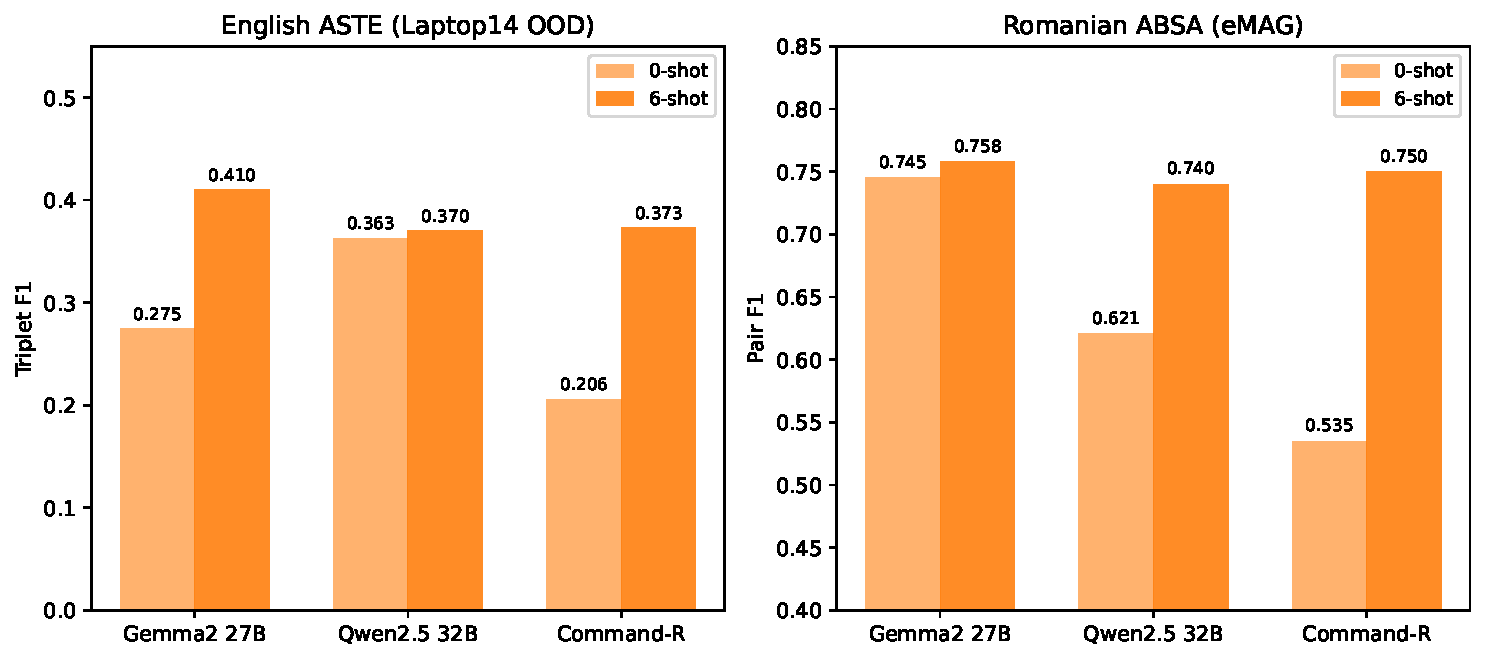
\includegraphics[width=0.95\textwidth]{figures/r4_llm_0shot_vs_6shot.pdf}
\caption{LLM performance in 0-shot vs 6-shot settings on English ASTE (left) and Romanian ABSA (right).}
\label{fig:0vs6}
\end{figure}


\section{In-Domain Benchmark Context}

To contextualise our OOD results, Table~\ref{tab:indomain-benchmark} shows in-domain performance when each dataset is trained and tested separately (the standard benchmark setup).

\begin{table}[H]
\centering
\caption{In-domain ASTE benchmark results (train and test on same dataset). Published results from original papers.}
\label{tab:indomain-benchmark}
\small
\begin{tabular}{@{}lcccc@{}}
\toprule
\textbf{Method} & \textbf{Rest14} & \textbf{Laptop14} & \textbf{Rest15} & \textbf{Rest16} \\
\midrule
\multicolumn{5}{l}{\textit{Discriminative (published)}} \\
\midrule
GTS (2020) & 70.92 & 59.46 & 62.53 & 68.71 \\
Span-ASTE (2021) & 72.89 & 62.40 & 64.45 & 71.85 \\
BTF-CCL (2025) & 75.88 & 63.29 & 67.68 & 73.80 \\
\midrule
\multicolumn{5}{l}{\textit{Generative (published)}} \\
\midrule
MvP (10-dataset multi-task) & 76.08 & 65.84 & 69.91 & 72.36 \\
\midrule
\multicolumn{5}{l}{\textit{Ours (per-dataset training)}} \\
\midrule
FLAN-T5 NL baseline & 72.4 & 62.7 & 64.0 & 72.5 \\
\bottomrule
\end{tabular}
\end{table}

Our per-dataset NL baseline is competitive with Span-ASTE across all four datasets and matches or exceeds GTS. It falls 3--4 points below BTF-CCL and MvP, both of which use specialised techniques. This confirms that our model is a reasonable representative of the generative ABSA approach.


\section{Error Analysis}\label{sec:errors}

We ran detailed error analysis on the NL baseline (seed 42) for both Rest14 (ID, F1 = 0.725) and Laptop14 (OOD, F1 = 0.542).

\subsection{Error Distribution}

\begin{table}[H]
\centering
\caption{Classification of missed gold triplets by whether the aspect/opinion terms appeared in training.}
\label{tab:errors-missed}
\small
\begin{tabular}{@{}lrrrr@{}}
\toprule
& \multicolumn{2}{c}{\textbf{Rest14 (ID)}} & \multicolumn{2}{c}{\textbf{Laptop14 (OOD)}} \\
\textbf{Missed type} & \textbf{Count} & \textbf{\%} & \textbf{Count} & \textbf{\%} \\
\midrule
Aspect unseen in training & 147 & 53.5 & 254 & 97.3 \\
Aspect seen in training & 128 & 46.5 & 7 & 2.7 \\
\midrule
Opinion unseen in training & 95 & 34.5 & 131 & 50.2 \\
Opinion seen in training & 180 & 65.5 & 130 & 49.8 \\
\bottomrule
\end{tabular}
\end{table}

The clearest evidence for why OOD performance drops: on Laptop14, 97.3\% of missed gold aspects are terms that never appeared in the restaurant training data (words like ``OS'', ``trackpad'', ``portability'', ``setup''). The model has no learned association between these tokens and the concept of ``aspect.'' Opinion terms show an even split (50.2\% unseen vs 49.8\% seen), consistent with the higher opinion token overlap.

\subsection{Element-Level Error Patterns}

\begin{table}[H]
\centering
\caption{Element-level error classification for unmatched predictions on Rest14 (ID) and Laptop14 (OOD). Percentages are relative to the total number of errors in each category.}
\label{tab:errors-element}
\small
\begin{tabular}{@{}lrrrr@{}}
\toprule
& \multicolumn{2}{c}{\textbf{Rest14 (ID)}} & \multicolumn{2}{c}{\textbf{Laptop14 (OOD)}} \\
\textbf{Error type} & \textbf{Count} & \textbf{\%} & \textbf{Count} & \textbf{\%} \\
\midrule
\multicolumn{5}{l}{\textit{Aspect errors}} \\
\midrule
Spurious & 81 & 57.4 & 115 & 81.6 \\
Boundary & 55 & 39.0 & 20 & 14.2 \\
Paraphrase & 4 & 2.8 & 1 & 0.7 \\
Hallucination & 1 & 0.7 & 5 & 3.5 \\
\midrule
\multicolumn{5}{l}{\textit{Opinion errors}} \\
\midrule
Spurious & 100 & 70.4 & 73 & 68.2 \\
Boundary & 42 & 29.6 & 33 & 30.8 \\
Hallucination & 0 & 0.0 & 1 & 0.9 \\
\midrule
\multicolumn{5}{l}{\textit{Polarity errors}} \\
\midrule
Wrong polarity & 130 & --- & 126 & --- \\
\bottomrule
\end{tabular}
\end{table}

Table~\ref{tab:errors-element} shows a notable shift in error composition between in-domain and out-of-domain evaluation. On Rest14, aspect boundary errors account for 39\% of aspect mistakes: the model identifies the correct region but disagrees on which words constitute the span (e.g., predicting ``grilled chicken'' where the gold is just ``chicken''). On Laptop14, boundary errors drop to 14.2\% while spurious errors rise from 57.4\% to 81.6\%: the model extracts real text that happens not to correspond to any annotated aspect. Many involve product names in aspect-like syntactic positions (``MBP'', ``Mac Mini'', ``Air'').

Opinion errors are more stable across domains (spurious: 70.4\% ID, 68.2\% OOD; boundary: $\sim$30\% both), consistent with opinion vocabulary being more transferable.

\subsection{Triplet-Level Error Patterns}

\begin{table}[H]
\centering
\caption{Triplet-level error patterns: which element combinations are wrong in unmatched predictions.}
\label{tab:errors-triplet}
\small
\begin{tabular}{@{}lrrrr@{}}
\toprule
& \multicolumn{2}{c}{\textbf{Rest14 (ID)}} & \multicolumn{2}{c}{\textbf{Laptop14 (OOD)}} \\
\textbf{Pattern} & \textbf{Count} & \textbf{\%} & \textbf{Count} & \textbf{\%} \\
\midrule
aspect+opinion+polarity & 70 & 25.9 & 71 & 33.0 \\
aspect only & 63 & 23.3 & 58 & 27.0 \\
opinion only & 63 & 23.3 & 26 & 12.1 \\
polarity only & 43 & 15.9 & 33 & 15.3 \\
aspect+polarity & 8 & 3.0 & 12 & 5.6 \\
opinion+polarity & 9 & 3.3 & 10 & 4.7 \\
duplicate & 14 & 5.2 & 5 & 2.3 \\
\bottomrule
\end{tabular}
\end{table}

Table~\ref{tab:errors-triplet} breaks down errors by which element combination is wrong. On in-domain data, the distribution is relatively even. On OOD data, opinion-only errors drop from 23.3\% to 12.1\% (opinion vocabulary transfers), while the all-three-wrong pattern rises to 33\%, representing cases where the model has pointed at an entirely unrelated part of the sentence.

\subsection{Polarity Confusion}

The most frequent polarity confusions on OOD data are: gold \textit{negative} predicted as neutral (21 cases), and gold \textit{positive} predicted as neutral (16 cases). Examining the actual sentences reveals that most ``neutral'' gold labels appear in desire/requirement contexts (``I needed a laptop with big storage'') or factual statements about missing features (``There is no HDMI receptacle''). The model predicts the polarity that surface-level words suggest rather than inferring the neutral pragmatic intent. The training distribution contributes: Rest14 has only 7\% neutral annotations, so the model has limited exposure to neutral contexts.

\subsection{Annotation Quality Issues}

A non-trivial fraction of ``errors'' reflect questionable gold annotations:

\begin{itemize}
    \item \textbf{Hypotheticals}: ``a spice rub \textit{might have} overwhelmed'' annotated as negative about spice rub, despite being a hypothetical dismissal.
    \item \textbf{Neutral in opinionated contexts}: ``There is no HDMI receptacle'' annotated neutral; model predicts negative (reporting a missing feature carries implicit dissatisfaction).
    \item \textbf{Desire context}: ``I needed a laptop with big storage, a nice screen and fast'' annotated neutral for ``big'' and ``nice''; model predicts positive for positive-valence adjectives.
\end{itemize}

We estimate 5--10\% of Laptop14 annotations involve genuinely ambiguous polarity where the model's prediction is at least as defensible as the gold label. This affects all methods equally and does not change relative comparisons.


\section{Discussion}

\subsection{Why Does NL Format Help OOD?}

The +8.6 point OOD improvement from NL format is the largest finding. We believe it works through two mechanisms:

\begin{enumerate}
    \item \textbf{Pre-training alignment}: FLAN-T5 was pre-trained to generate fluent English. The NL templates are within the model's pre-training distribution. On OOD inputs where the model is uncertain, it can still generate well-formed template text. The structured format is an arbitrary syntax that provides no such fallback.
    
    \item \textbf{Implicit structural constraints}: The template words act as barriers against degenerate outputs. A model generating structured output can easily produce malformed brackets when uncertain. The NL template's connecting phrases force complete triplets or nothing recognisable.
\end{enumerate}

The evidence against a third hypothesis, that NL simply provides more training signal through longer outputs, is that strategies which increase training volume (sub-task decomposition, multi-ordering) do not show similar gains. The benefit is specifically from output-side alignment with pre-training.

\subsection{Why Do Most Interventions Fail?}

The negative results share a common pattern: interventions that increase training variety \textit{within the same domain} do not help when the test domain has fundamentally different vocabulary and annotation style. Curriculum learning, sub-task decomposition, masking, and multi-ordering all produce more diverse training examples, but the diversity is over task structure, not over domain content.

Cross-domain data mixing is the one intervention that adds actual domain diversity, yet it still fails for far-OOD. The DMASTE domains are more similar to each other (Amazon product reviews) than to the SemEval restaurant domain. Adding more Amazon-style data does not bridge the gap to laptop reviews annotated in SemEval style.

\subsection{Annotation Quality and Performance Ceiling}

Evaluating models on benchmark data assumes that the gold annotations represent ground truth. In practice, annotation is subjective: Miñarro-Giménez et al.~\cite{minarro2019quantitative} demonstrated that even trained annotators show non-trivial disagreement on structured labelling tasks. Hu and Liu~\cite{hu2004mining}, in their early work on opinion mining, acknowledged that identifying what constitutes an opinion is inherently context-dependent. Li et al.~\cite{li2021implicit} showed that neural language models develop implicit representations of entity state from text alone, but these representations are imperfect. Sun et al.~\cite{sun2025implicit} argue that text embedding research should move beyond surface meaning toward modelling implicit semantics, precisely the kind of pragmatic inference needed to correctly handle ambiguous polarity cases.

For the English SemEval data, we estimate that 5--10\% of Laptop14 annotations involve genuinely ambiguous polarity. The annotation guidelines leave room for interpretation in cases involving implicit sentiment, pragmatic inference, and debatable polarity. The distinction between surface semantics and implicit meaning is at the core of many ``errors'': the model, trained on surface-level aspect-opinion-polarity annotations, predictably struggles with cases where the correct label requires understanding speech acts, pragmatic implicature, or counterfactual reasoning.

For the Romanian dataset specifically, the GPT-4 annotation pipeline introduces additional concerns:
\begin{itemize}
    \item Category assignment is the most annotation-sensitive component. The boundary between categories like ``experience'' and ``performance'', or ``design'' and ``durability'', requires domain expertise and subjective judgement that GPT-4 may resolve differently from a human annotator.
    \item There is an inherent circularity concern: models are trained on LLM-annotated data and then compared against LLMs on test data from a related pipeline. We mitigate this by using an independently annotated test set, but biases in the training set still propagate to all fine-tuned models.
    \item The quality ceiling is bounded by GPT-4's ability to perform fine-grained Romanian ABSA. Aldeen et al.~\cite{aldeen2023chatgpt} found that LLM-generated annotations achieve competitive quality for sentiment classification but human annotators consistently outperform on tasks requiring nuanced contextual judgement.
\end{itemize}

The practical consequence is that reported F1 scores on both datasets should be interpreted with caution. The gap between model performance and ``perfect'' F1 is not entirely due to model limitations; a portion reflects genuine annotation ambiguity. Importantly, this annotation noise affects all methods equally: relative comparisons between models remain valid even if absolute F1 scores overstate the difficulty.



\chapter{Conclusions}\label{ch:conclusions}

This chapter summarises the findings of the thesis, acknowledges the limitations of the experimental setup, and outlines directions for future research.

\section{Summary}

This thesis presented a systematic empirical study of training strategies for out-of-domain generalisation in generative aspect-based sentiment analysis. We evaluated output format, syntactic enrichment, multiple data augmentation strategies, task decomposition methods, decoding strategies, large language models in few-shot settings, and application to Romanian, measuring their OOD impact with multi-seed statistical validation across three benchmarks.

The main finding is that natural-language output format is the single most effective lever for OOD generalisation, providing +8.6 F1 points over structured output with non-overlapping confidence intervals. This is a design choice that costs nothing in terms of additional data or computation, yet delivers larger OOD gains than any other intervention we tested.

On the DMASTE benchmark, our FLAN-T5-base model with NL output matches the best previously reported cross-domain result (Span-ASTE) without any domain adaptation. On the SemEval benchmark, it outperforms 27--32B parameter LLMs in few-shot settings by 10+ F1 points on OOD data.

On Romanian ABSA, fine-tuned models (110--278M parameters) outperform all LLMs tested (27--35B parameters). Monolingual Romanian models perform within 0.3 F1 points of the 2.5$\times$ larger multilingual XLM-R, confirming that dedicated language-specific pre-training compensates for smaller model size.

Most other interventions we tested, syntactic enrichment, curriculum learning, aspect masking, cross-domain data mixing, LLM-generated opinion augmentation, training with permuted task orderings (and a faithful replication of MvP's inference-time voting~\cite{gou2023mvp}), sub-task decomposition~\cite{xie2025star}, and alternative decoding strategies, did not reliably improve OOD performance. These negative results are documented in detail so that future work can avoid repeating them.

\section{Limitations}

This work has several limitations:

\begin{itemize}
    \item \textbf{Single language family for ASTE}: All triplet extraction experiments are in English. The Romanian experiments use a different task formulation (polarity+category, not full triplets), so we cannot confirm that the NL format advantage extends to non-English triplet extraction.
    
    \item \textbf{Single model size}: We tested only FLAN-T5-base (250M). It is possible that the NL format advantage diminishes at larger scales where the model has more capacity to learn arbitrary output formats.
    
    \item \textbf{Annotation noise ceiling}: The SemEval benchmarks contain annotation inconsistencies that affect all methods equally but make it difficult to determine the true performance ceiling.
    
    \item \textbf{Single-seed for some experiments}: While the primary comparisons use 5 seeds, several ablation studies use a single seed due to computational constraints. Results within the baseline's confidence interval cannot be conclusively interpreted.
    
    \item \textbf{DMASTE implicit aspects}: The DMASTE datasets have 40--47\% implicit aspects which our model handles but cannot truly solve; predicting aspects not mentioned in the text is a fundamentally different problem from extracting mentioned spans.
    
    \item \textbf{LLM quantisation}: All LLMs are 4-bit quantised, which reduces performance relative to full-precision inference. Results represent a lower bound on LLM capability.
    
    \item \textbf{Romanian annotation quality}: The eMAG training data was annotated with GPT-4 assistance, which may introduce systematic biases bounded by GPT-4's capabilities on Romanian text.
\end{itemize}

\section{Future Work}

Several directions could extend this work:

\begin{itemize}
    \item \textbf{Implicit aspect generation}: Using LLMs to rewrite sentences with explicit aspects into versions with implied aspects, then training on both. This would directly address the implicit aspect gap that explains much of the DMASTE difficulty.
    
    \item \textbf{Domain-adaptive pre-training}: Continuing FLAN-T5's pre-training on unlabeled target-domain text before fine-tuning on labeled source-domain data. This could address the vocabulary gap without requiring labeled target data.
    
    \item \textbf{Larger model scales}: Testing whether the NL format advantage persists with FLAN-T5-large (780M) or T5-XL (3B), and whether the augmentation strategies that failed at 250M become effective with more capacity.
    
    \item \textbf{Multi-task cross-domain training}: Combining NL output format with MvP-style multi-dataset training. If multi-task exposure provides domain diversity, it might compound with the NL format's OOD advantage.
    
    \item \textbf{Better augmentation targets}: Our augmentation attempts modified opinions (synonym replacement) and inputs (masking, data mixing). Augmenting the aspects themselves, generating training sentences with novel aspect terms from target-domain vocabulary, could address the unseen-aspect problem that accounts for 57\% of OOD errors.
    
    \item \textbf{Fine-tuning smaller LLMs}: Testing 7--8B parameter models fine-tuned on ABSA to find the scale at which fine-tuned LLMs begin to outperform fine-tuned smaller models.
    
    \item \textbf{Romanian triplet extraction}: Expanding Romanian ABSA evaluation to full ASTE rather than polarity+category classification.
\end{itemize}


\chapter{Annex}\label{ch:annex}

\section{Per-Seed Results}

\begin{table}[H]
\centering
\caption{NL baseline: per-seed triplet F1 on all test sets (Rest14-only training).}
\small
\begin{tabular}{@{}ccccc@{}}
\toprule
\textbf{Seed} & \textbf{Rest14} & \textbf{Rest15} & \textbf{Rest16} & \textbf{Laptop14} \\
\midrule
42 & 0.727 & 0.607 & 0.672 & 0.543 \\
123 & 0.718 & 0.598 & 0.688 & 0.517 \\
456 & 0.717 & 0.603 & 0.672 & 0.520 \\
789 & 0.727 & 0.600 & 0.690 & 0.532 \\
1337 & 0.720 & 0.603 & 0.677 & 0.512 \\
\midrule
Mean & 0.722 & 0.602 & 0.680 & 0.525 \\
Std & 0.005 & 0.004 & 0.010 & 0.012 \\
\bottomrule
\end{tabular}
\end{table}

\begin{table}[H]
\centering
\caption{Structured baseline: per-seed triplet F1 (Rest14-only training).}
\small
\begin{tabular}{@{}ccccc@{}}
\toprule
\textbf{Seed} & \textbf{Rest14} & \textbf{Rest15} & \textbf{Rest16} & \textbf{Laptop14} \\
\midrule
42 & 0.698 & 0.570 & 0.637 & 0.421 \\
123 & 0.684 & 0.580 & 0.640 & 0.441 \\
456 & 0.694 & 0.565 & 0.632 & 0.449 \\
789 & 0.701 & 0.582 & 0.651 & 0.441 \\
1337 & 0.686 & 0.577 & 0.640 & 0.444 \\
\midrule
Mean & 0.693 & 0.575 & 0.640 & 0.439 \\
Std & 0.008 & 0.009 & 0.009 & 0.012 \\
\bottomrule
\end{tabular}
\end{table}

\section{Example Model Outputs}

\textbf{Correct extraction (ID, Rest14):}
\begin{lstlisting}
Input: Great food but the service was dreadful !
Output: food is described as Great, expressing a positive sentiment ;
        service is described as dreadful, expressing a negative sentiment
\end{lstlisting}

\textbf{OOD error --- unseen aspect (Laptop14):}
\begin{lstlisting}
Input: This Macbook Pro is fast, powerful, and runs super quiet and cool.
Gold: runs -> quiet [positive] ; runs -> cool [positive]
Pred: Macbook Pro -> fast [positive] ; Macbook Pro -> powerful [positive] ;
      Macbook Pro -> quiet [positive] ; Macbook Pro -> cool [positive]
\end{lstlisting}
The model identifies the product name as the aspect rather than the verb ``runs''. This reflects different annotation conventions between restaurant and laptop domains.

\textbf{OOD error --- polarity confusion (Laptop14):}
\begin{lstlisting}
Input: I needed a laptop with big storage, a nice screen and fast ...
Gold: storage -> big [neutral] ; screen -> nice [neutral]
Pred: storage -> big [positive] ; screen -> nice [positive]
\end{lstlisting}
Desire/wish context should be neutral per annotation guidelines, but the model defaults to positive for positive-sounding adjectives.

\section{Input/Output Format Examples}

\textbf{Full prompt with compact dependency annotations:}
\begin{lstlisting}
Task: aspect-extraction, sentiment-extraction, polarity-inference
Input: The staff was so horrible to us .
Syntax: staff->was:nsubj horrible->was:acomp
Output: staff is described as horrible, expressing a negative sentiment
\end{lstlisting}

\textbf{Structured output for the same input:}
\begin{lstlisting}
Task: aspect-extraction, sentiment-extraction, polarity-inference
Input: The staff was so horrible to us .
Output: [staff, horrible, negative]
\end{lstlisting}


\section{Multi-Ordering Template Permutations}\label{sec:annex-templates}

The 6 natural-language templates used for multi-ordering training on the full ASTE triplet task:

\begin{table}[H]
\centering
\caption{NL output templates for all 6 element orderings of the ASTE triplet.}
\small
\begin{tabular}{@{}lp{10.5cm}@{}}
\toprule
\textbf{Task prefix order} & \textbf{Template} \\
\midrule
aspect, sentiment, polarity & \texttt{\{aspect\} is described as \{sentiment\}, expressing a \{polarity\} sentiment} \\
aspect, polarity, sentiment & \texttt{\{aspect\} carries a \{polarity\} opinion, expressed as \{sentiment\}} \\
sentiment, aspect, polarity & \texttt{the opinion \{sentiment\} is expressed towards \{aspect\}, conveying a \{polarity\} sentiment} \\
sentiment, polarity, aspect & \texttt{\{sentiment\} conveys a \{polarity\} sentiment about \{aspect\}} \\
polarity, aspect, sentiment & \texttt{a \{polarity\} sentiment toward \{aspect\} is expressed as \{sentiment\}} \\
polarity, sentiment, aspect & \texttt{a \{polarity\} sentiment is expressed as \{sentiment\}, regarding \{aspect\}} \\
\bottomrule
\end{tabular}
\end{table}


\section{Per-Model LLM Results (English)}

\begin{table}[H]
\centering
\caption{Gemma2 27B detailed results (SemEval ASTE, triplet micro-F1).}
\small
\begin{tabular}{@{}lcccc@{}}
\toprule
\textbf{Setting} & \textbf{Rest14} & \textbf{Rest15} & \textbf{Rest16} & \textbf{Laptop14} \\
\midrule
0-shot & 0.441 & 0.418 & 0.455 & 0.275 \\
6-shot & 0.646 & 0.592 & 0.637 & 0.410 \\
\bottomrule
\end{tabular}
\end{table}

\begin{table}[H]
\centering
\caption{Qwen2.5 32B detailed results (SemEval ASTE, triplet micro-F1).}
\small
\begin{tabular}{@{}lcccc@{}}
\toprule
\textbf{Setting} & \textbf{Rest14} & \textbf{Rest15} & \textbf{Rest16} & \textbf{Laptop14} \\
\midrule
0-shot & 0.535 & 0.451 & 0.556 & 0.363 \\
6-shot & 0.603 & 0.527 & 0.614 & 0.370 \\
\bottomrule
\end{tabular}
\end{table}

\begin{table}[H]
\centering
\caption{Command-R detailed results (SemEval ASTE, triplet micro-F1).}
\small
\begin{tabular}{@{}lcccc@{}}
\toprule
\textbf{Setting} & \textbf{Rest14} & \textbf{Rest15} & \textbf{Rest16} & \textbf{Laptop14} \\
\midrule
0-shot & 0.318 & 0.256 & 0.309 & 0.206 \\
6-shot & 0.576 & 0.499 & 0.568 & 0.373 \\
\bottomrule
\end{tabular}
\end{table}


\section{LLM Prompt Templates}

\textbf{English ASTE (6-shot format):}
\begin{lstlisting}
[system]
You are an aspect-based sentiment analysis system. Given a review
sentence, extract all (aspect, opinion, polarity) triplets.

Output format: one triplet per line as [aspect, opinion, polarity]
- aspect: the entity or feature being discussed (exact span from text)
- opinion: the opinion expression about the aspect (exact span from text)
- polarity: positive, negative, or neutral

If there are no triplets, output: none
Do not explain your reasoning. Only output the triplets.

[user]
Input: The price is reasonable although the service is poor .

[assistant]
[price, reasonable, positive]
[service, poor, negative]

... (5 more examples) ...

[user]
Input: The design and atmosphere is just as good .
\end{lstlisting}

\textbf{Romanian ABSA (6-shot format):}
\begin{lstlisting}
[system]
You are a sentiment analysis system for phone reviews written in
Romanian. Given a review, extract all (category, polarity) pairs.

Output format: one pair per line as [category, polarity]
- category: Must be one of: experience, durability, performance,
  battery, price_quality, design, camera, audio, software, brand,
  service
- polarity: Must be one of: positive, negative, neutral

If there are no pairs, output: none
Do not explain your reasoning. Only output the pairs.

[user]
Input: Nu merita. Se incalzeste tare.

[assistant]
[experience, negative]
[performance, negative]
[price_quality, negative]

... (5 more examples) ...

[user]
Input: Super telefon pentru cei cunoscatori!
\end{lstlisting}


\addcontentsline{toc}{chapter}{Bibliography}
\bibliographystyle{plain}
\bibliography{bibliographyDizertatie}

\end{document}
